\documentclass[11pt]{book}
% Packages are in alphabetical order, the only exceptions are made to avoid import conflicts.  

\usepackage[x11names]{xcolor}% Color extensions, import first to avoid package conflicts
%\usepackage[T1]{fontenc}
\usepackage[sfdefault]{universalis}
\DeclareFontFamilySubstitution{TS1}{UniversalisADFStd(0)}{cmr}
\usepackage[margin=1in]{geometry}% Formatting on page
\usepackage{array}% big arrays
\usepackage{amsmath}% Math symbols
\usepackage{amsthm}%   
\usepackage{amssymb}%
\usepackage[backend=biber]{biblatex} % bibliography
\usepackage{bm}% bold, even for greek letters
\usepackage{cancel}% slash or x out text or equations
\usepackage[format=hang]{caption}
\usepackage{enumitem}% Enumerating things, more flexible than itemize
\usepackage{esint}% better double and triple Integrals
\usepackage{etoc}% Flexibly designed table of contents
\usepackage{fancyhdr} % Headers
    \pagestyle{fancy}%
\usepackage{float}% Position figures and tables flexibly
\usepackage{subfloat}
\usepackage{subfig}
\usepackage{gensymb}%
\usepackage{graphicx}% plots and graphics
\usepackage{listings}% type code, autosets colors for different languages
\usepackage{mathcommand}% Allows for macros to be defined differently in math environments.
\usepackage{pgfplots}% plots and graphics
	\pgfplotsset{compat=newest} % or use compat=1.6
	\usepgfplotslibrary{fillbetween}%
	\usepgfplotslibrary{statistics}% for histograms
\usepackage{physics}% Predefined commands for many physics things
\usepackage{slashed}
\usepackage{relsize}% Allows for larger/smaller math 
\usepackage{textcomp}% Gets rid of perthousand error
\usepackage{tikz}% Pictures
	\usetikzlibrary{decorations.markings}%
	\usetikzlibrary{3d,calc,fadings,patterns,intersections}%
	\usetikzlibrary{datavisualization.formats.functions}%
	\usetikzlibrary{decorations.pathmorphing}%
	\usetikzlibrary{decorations.text}%
\usepackage{tcolorbox}% Beautiful colored boxed with flexible options
	\tcbuselibrary{xparse, skins}
\usepackage{upquote}% Fixes quotes in verbatim environment
\usepackage{verbatim}% Defines the "comment" environment
\usepackage{wrapfig}% 
\usepackage[final]{pdfpages}
\usepackage{xparse}% Allows for more flexible command definitions 
\usepackage[compat=1.1.0]{tikz-feynman}% Feynman diagrams
\usepackage{xspace}
\usepackage[hidelinks]{hyperref}% References--Put this last for compatability

\endinput
% Custom macros that I use in Physics and Math Documents
% The order of this document is:
%	Document structure/document style (I don't use .sty because I haven't figured out how to make it compatibile with VSC)
%	Physics shorthand commands
%	Math shorthand and symbols

%%%% Document Structure %%%%
	% Creates a bolded title that is a hypertarget with link="top", optional bolded subtitle that's scaled properly 
	\NewDocumentCommand\thetitle{m O{}}{ \title{ \hypertarget{top}{\textbf{#1}} \\ \large {#2} } }
	
	% University of Michigan Colors
	\definecolor{WolverineMaize}{cmyk}{0,0.18,1,0}
	\definecolor{WizardGreen}{RGB}{21, 110, 45}
	\definecolor{WolverineBlue}{cmyk}{1,0.69,0,0.6}
	\definecolor{UMMATan}{cmyk}{0.06, 0.14, 0.39, 0.08}
	\definecolor{BurtonTowerBeige}{cmyk}{0.21, 0.15, 0.54, 0.31}
	\definecolor{TappanRed}{cmyk}{0.08, 0.92, 1.00, 0.33}
	% ATLAS Colors
	\definecolor{ATLASBlue}{RGB}{11,128,195}
	\def\UM{\colorbox{WolverineBlue}{\textcolor{WolverineMaize}{\textbf{University of Michigan}}}}% School Pride

	\def\EC{\href{https://github.com/CarpenterEvan/PhysicsReview}{\(\mathbb{E}\textsc{van}~\mathbb{C}\textsc{arpenter}\)}}

	\numberwithin{equation}{section} % amsmath command that renews equation counter in each section\
	\DeclareTotalTColorBox{\mymathbox}{m m}{
		bicolor,
		colframe=WolverineBlue,
		colback=WolverineMaize,
		float=h,
		drop shadow,
		every float=\centering,
		title=#1, 
		width=0.66\pdfpagewidth,
		}{#2}

	\DeclareTColorBox{mathbox}{m}{
		colframe=WolverineBlue,
		colback=WolverineMaize,
		float=h,
		every float=\centering,
		title=#1, 
		width=0.75\textwidth,
		}
%%
%%
%%%% Physics %%%%
	%%
	%% Transverse Quantities
		\NewDocumentCommand{\pT}{}{$p_{\rm T}$} % transverse momentum
		\NewDocumentCommand{\ET}{}{$E_{\rm T}$} % transverse Energy
		\NewDocumentCommand{\MET}{}{$E_{\rm T}^{\rm miss}$} % transverse Energy

	%%
	%% Particles
		\NewDocumentCommand{\h}{s}{\IfBooleanTF{#1}{\(H\)}{\(H^0\)}}
		\NewDocumentCommand{\Z}{s}{\IfBooleanTF{#1}{\(Z\)}{\(Z^0\)}}
		\NewDocumentCommand{\W}{s O{+}}{\IfBooleanTF{#1}{\(W^{#2}\)}{\(W^{\pm}\)}}
		
	\def\ik{4\pi\epsilon_0} % Inverse k for EM
	%%
%%
%%
%%%% Math %%%%
	%%
	%% Symbols and Shorthand
		% to make sets
		\LoopCommands{\lettersAll}[#1set] {\newmathcommand#2{\{\MakeUppercase{#1}\}}}% \Qset --> {Q}
		\LoopCommands{\lettersAll}[#1set] {\newtextcommand#2{\(\MakeUppercase{#1}\)}}% set command but math mode
		\LoopCommands{\lettersAll}[#1hat] {\newmathcommand#2{\hat{#1}}}%
		\def\placeholder{\bm{\,\cdot\,}}% Placeholder of the argument of a function
		\def\ints{\int_\mathcal{S}}% Surface integral
		\def\intv{\int_{D}}% Volume integral with D subscript
		\def\intall{\int_{-\infty}^{\infty}}% Integral over all space
		\def\iintall{\iint_{\rm All Space}}% Integral over all space
		\def\iiintall{\iiint_{\rm All Space}}% Integral over all space
		\def\lap{\mathcal{L}}% Laplace
		\NewDocumentCommand{\e}{s m}{% Basis vector
		% \e{x} --> \hat{e}_x
		% \e*{x} --> \hat{x}
		% e, x will be bolded, even if x is greek letter.
		\IfBooleanTF{#1}
		{\mathbf{\hat{e}_{#2}}}
		{\bm{\hat{#2}}}}
		\ExplSyntaxOn
		% Helper macro to safely strip the backslash from a macro token for \csname
		\newcommand{\stripbackslash}[1]{\expandafter\@gobble\string#1}
		\ExplSyntaxOff
		
		\NewDocumentCommand\slsh{m}{\slashed{#1}}
		% Integral differentials
			% Vector differentials like \dl, \da come by default with dot product \cdot, 
			% Hide \cdot with * option (\dl*, \da*)
			\def\d{{\rm d}}% for integration
			\NewDocumentCommand{\dl}{s}{
				\,\d\bm{\ell}
			}
			\NewDocumentCommand{\da}{}{
				\,\d\bm{a}
			}
			\LoopCommands{fqrstVxyz}[d#1]{\NewDocumentCommand#2{s}{\,\d#1}}
			\NewDocumentCommand\dphi{}{\,\d{\phi}}
			\NewDocumentCommand\dtheta{}{\,\d{\theta}}

		\NewDocumentCommand\oo{O{1} m}{\frac{#1}{#2}}% reciprocal- 'one over', optional argulent is there to make it a regular fraction, because oo is still quicker to type.
	%%
	%% Vectors and Matrices
		\NewDocumentCommand{\parametric}{m}{% Don't trust the highlighting, this has the correct number of curly braces.
			% Makes a matrix with "{" on the left and nothing on the right
			% useful for parametric definitions.
		    \left\{ 
			\begin{gathered}
				\begin{matrix}
					#1
		    	\end{matrix}
			\end{gathered}
			\right.
		}

		\NewDocumentCommand{\colvec}{+m}{% Colummn vector
			\begingroup
				\renewcommand{\arraystretch}{1.25}% I like it to have slightly more space (default=1.2)
				\begin{gathered}
					\begin{bmatrix}
						#1
					\end{bmatrix}
				\end{gathered}
			\endgroup
		}
	%%
	%% Derivatives
		\NewDocumentCommand{\der}{s O{} m g}{% custom derivative command
			% \der*{x}          --> D_x
			% \der[2]{x}        --> d^{2}f/d^{2}x
			% \der{x}           --> d/dx
			% \der{f}{x}		--> df/dx
			% \der{f}{x}{y}		--> (df/dx)_{y}
			% \der[a]{f}{x}{y}	--> (d^{a}f/dx^{a})_{y}
			% \der*[a]{b}{c}{e}	--> (D^{a}_{c} b)_{e}
			\IfBooleanTF{#1}
			{\IfNoValueTF{#4}% g returns -NoValue- if no argument
				{\mathrm{D}_{#3}^{#2}}
				{\mathrm{D}_{#4}^{#2}#3}
			}
			{\IfNoValueTF{#4}
				{\frac{\mathrm{d}^{#2}}{\mathrm{d} #3^{#2}}}
				{\frac{\mathrm{d}^{#2} #3}{\mathrm{d} #4^{#2}}}
			}
		}
		\NewDocumentCommand{\pder}{s O{} m g d[]}{% custom partial derivative command, 
			% \pder*{x} 		--> ∂_x
			% \pder[2]{x}		--> ∂^{2}f/∂^{2}x
			% \pder{x}			--> ∂/∂x
			% \pder{f}{x}		--> ∂f/∂x
			% \pder{f}{x}{y}	--> (∂f/∂x)_y
			% \pder*[a]{b}{c}[e]--> (∂^{a}_{c} b)_{e}
			% \pder[a]{b}{c}[e]--> (∂^{a}b/∂^{a}c)_{e}
			\IfBooleanTF{#1}
			{\IfNoValueTF{#4} 
				{\partial_{#3}^{#2}}
				{\partial_{#4}^{#2}#3}
					}
			{\IfNoValueTF{#5}% d[] returns -NoValue- if no argument present delimited by []
				{\IfNoValueTF{#4}
					{\frac{\partial^{#2}}{\partial#3^{#2}}}
					{\frac{\partial^{#2} #3}{\partial#4^{#2}}}
				}{
					{\IfNoValueTF{#4} 
					{\left(\frac{\partial^{#2}}{\partial#3^{#2}}\right)_{\!#5}\!\!}% \! is negative \, space
					{\left(\frac{\partial^{#2} #3}{\partial#4^{#2}}\right)_{\!#5}\!\!}}
				}
			}
		} 
			
	%%
	%% Misc. Problem Solving
		\NewDocumentCommand{\coloredanswer}{O{LavenderBlush2} m}{% makes coloredbox with pretty color
		\mathchoice{% Allows for different styles depending on the math mode.
				\colorbox{#1}{$\displaystyle #2$}
			}{
				\colorbox{#1}{$\textstyle #2$}}
		{}
		{}}
		\newcounter{probcount}% new counter for problem numbers, starts at 0 by default
		\NewDocumentEnvironment{ problem } {O{} +b}% Problem environment for homework, autocounts numbers, behaves like a section and can get listed (and hyperlinked) in the toc. 
			{\addtocounter{probcount}{1}% increase counter at the beginning of every problem
			\phantomsection% invisible page marker for hyperref
			\addcontentsline{toc}{subsection}{Problem \theprobcount~{\it#1}}% add "Problem \theprobcount. \textit{#1}" to table of contents (toc) as if it were a subsection
			\begin{trivlist}% begin unmarked ("trivial") list
			\item {\bf Problem \theprobcount} {\it#1}% print Problem with the counter and optional text 
			\item #2% +b is for inputs that are long
			\end{trivlist}% end list
			}{}% don't do anything, then "problem" environment ends, irrelevant because trivlist is already ended
	%%

\endinput
\addbibresource{references.bib}
\begin{document}
\tableofcontents
\chapter{Theory (Bachelors/Masters)}
	\section{Linear Algebra}
		\subsection{Algebraic Objects and Operations}
	\mymathbox{Set}{
		\begin{align*}
			\{S\}
		\end{align*}
		Requirements:
		\(\varnothing\in\{S\}\)
	}
	A set is a collection of objects. It could be numbers, bugs, words, functions, it really doesn't matter.
	Examples:
	\begin{align*}
		\{S_1\} &= \{1,2,3,4,\ldots\}
		\\
		\{S_2\} &= \{a,b,c,d\}
		\\
		\{S_3\} &= \{\{S_1\}, \{S_2\}\}
		\\
		\{\text{birds}\} &= \{\text{pigeons},\,\text{crows},\,\text{penguins},\,\text{emus}\}
	\end{align*}
	\begin{figure}[H]
		\centering
		\subfloat{
			\begin{tikzpicture}[scale=1.3]
				\node (O) at (0,0) {};
				\coordinate (S_4) at ($(O)+(0,1)$);
				\filldraw[fill=blue!10!white, decoration={random steps, segment length=5, amplitude=2}] (S_4)
				decorate { to[bend left] ++ (90:2)  }
				decorate { to[bend left] ++ (90:1)   }
				decorate { to[bend left] ++ (0:1)   }
				decorate { to[bend left] ++ (2,0)    }
				decorate { to[bend left] ++ (0.5,-2) }
				decorate { to[bend left] (S_4) };
				\node at ($(S_4)+(0.5,2.5)$)   {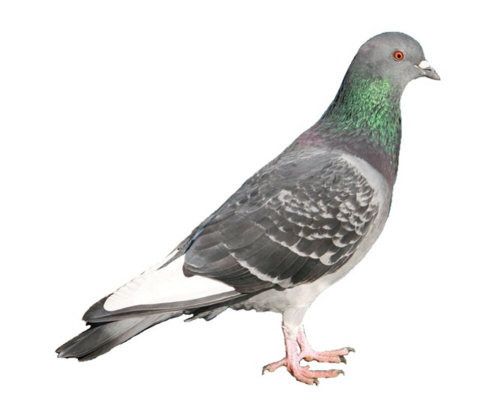
\includegraphics[width=1.3cm]{images/pigeon.png}};
				\node at ($(S_4)+(0.5,0.75)$)  {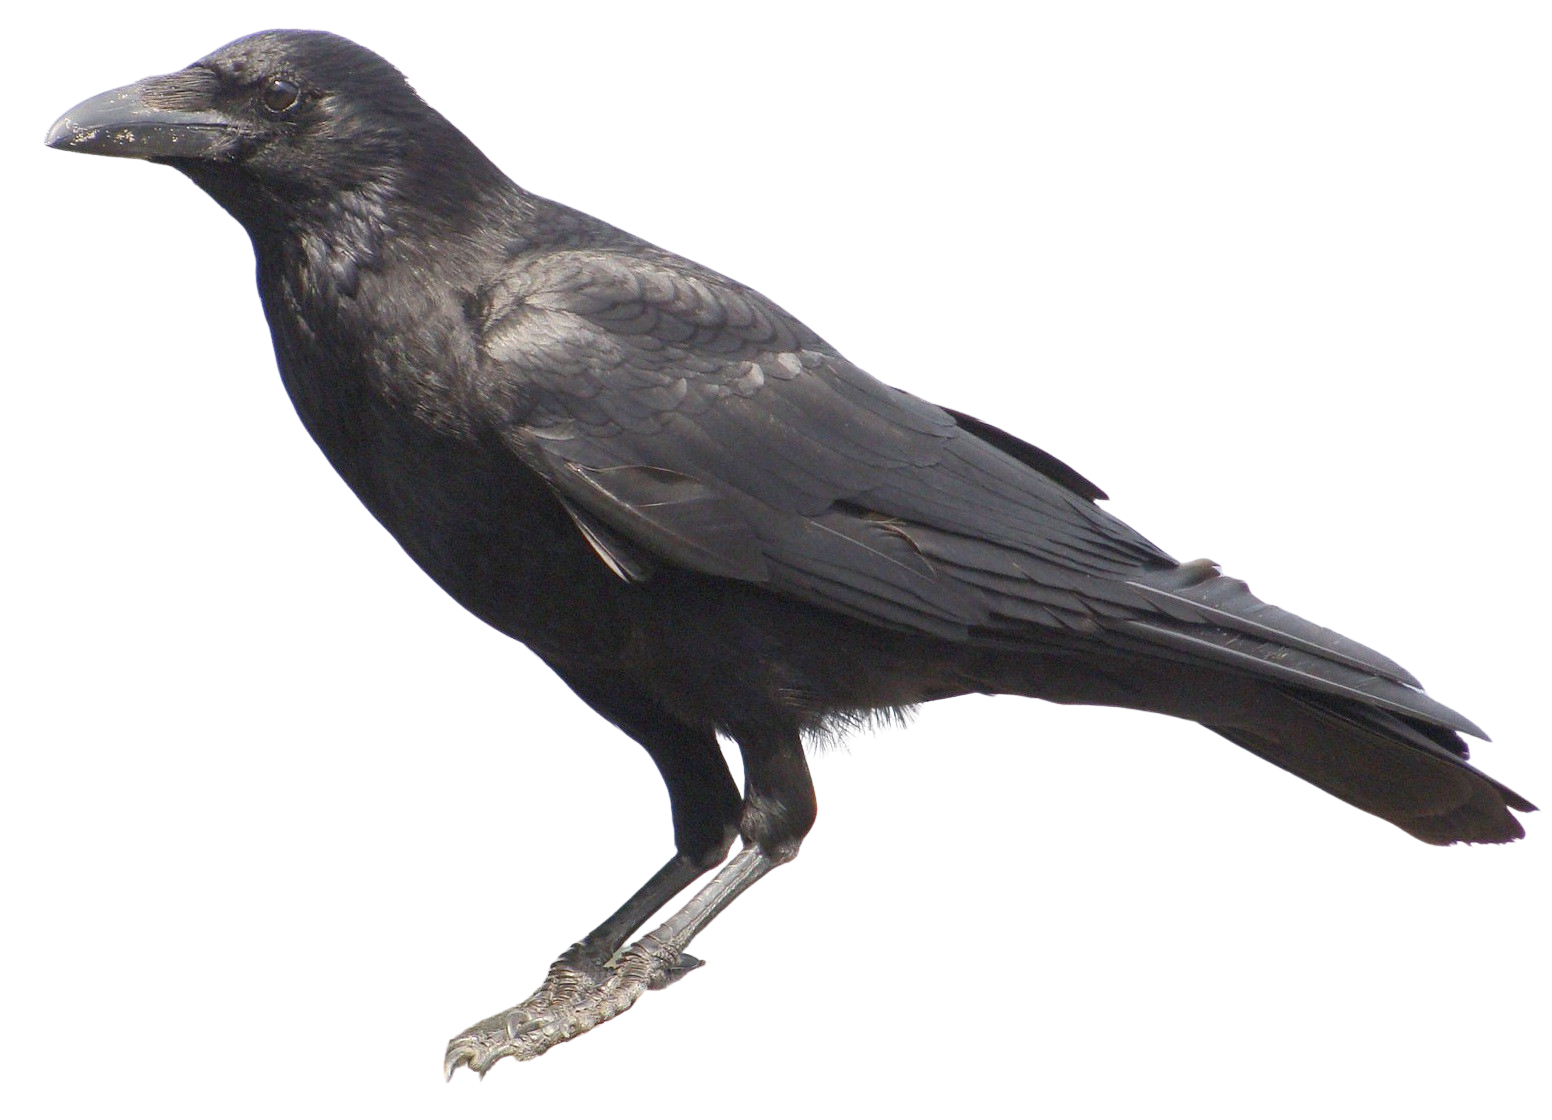
\includegraphics[width=1.3cm]{images/crow.png}};
				\node at ($(S_4)+(2.5,1.75)$)  {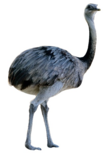
\includegraphics[width=1.3cm]{images/rhea.png}};
				\node at ($(S_4)+(1.35,1.25)$) {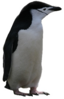
\includegraphics[width=0.8cm]{images/penguin.png}};
				\node at ($(S_4)+(1.75,-1)$) {birds};
			\end{tikzpicture}
		}
		\hfill
		\subfloat{
			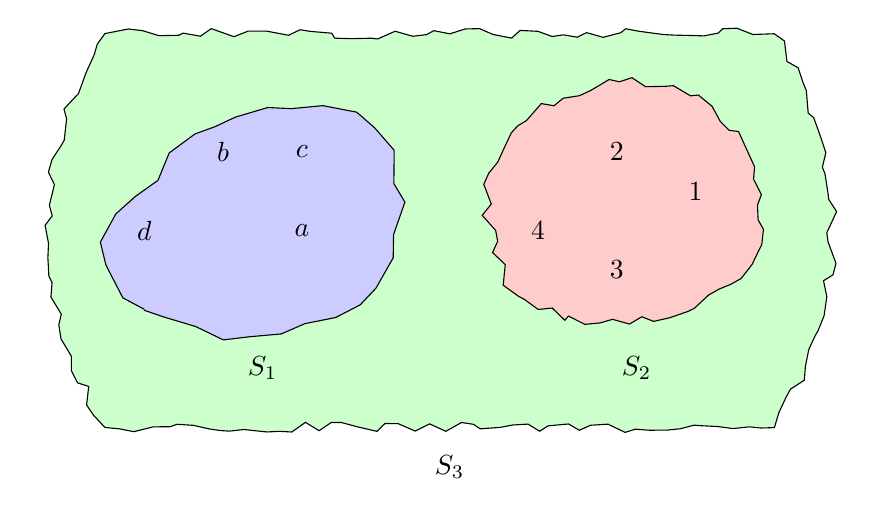
\begin{tikzpicture}
				\filldraw[fill=green!20, decoration={random steps, segment length=5, amplitude=2}] (-0.5,-1.5)
				decorate { to[bend left] (-0.5,3.5) }
				decorate { -- (8,3.5) }
				decorate { to[bend left] (8,-1.5) }
				decorate { -- (-0.5,-1.5) };
				\coordinate (S_1) at (0,0);
				\filldraw[fill=blue!20, decoration={random steps}] (S_1)
				decorate { to[bend left] ++ (120:1) }
				decorate { to[bend left] ++ (45:1)  }
				decorate { to[bend left] ++ (45:1)  }
				decorate { to[bend left] ++ (2,0)   }
				decorate { to[bend left] ++ (0,-2)  }
				decorate { to [bend left] (0,0)     };
				\node at ($(S_1)+(2,1)$) {\(a\)};
				\node at ($(S_1)+(1,2)$) {\(b\)};
				\node at ($(S_1)+(0,1)$) {\(d\)};
				\node at ($(S_1)+(2,2)$) {\(c\)};
				\node (S_1_Label) at ($(S_1)+(1.5,-0.75)$) {\(S_1\)};
				\coordinate (S_2) at (5,0);
				\filldraw[fill=red!20, decoration={random steps, segment length=5, amplitude=2}] (S_2)
				decorate { to[bend left] ++ (120:1)  }
				decorate { to[bend left] ++ (90:1)   }
				decorate { to[bend left] ++ (45:1)   }
				decorate { to[bend left] ++ (2,0)    }
				decorate { to[bend left] ++ (0.5,-2) }
				decorate { to[bend left] (S_2) };
				\node at ($(S_2)+(2,1.5)$) {\(1\)};
				\node at ($(S_2)+(1,2)$)   {\(2\)};
				\node at ($(S_2)+(1,0.5)$) {\(3\)};
				\node at ($(S_2)+(0,1)$)   {\(4\)};
				\node (S_2_Label) at ($(S_2)+(1.25,-0.75)$) {\(S_2\)};
				\node at ($(S_1_Label)!0.5!(S_2_Label)-(0,1.25)$) {\(S_3\)};
			\end{tikzpicture}
			}
			\caption{Sets can be anything.}
	\end{figure}
	Sets can be split into different subsets based on some definition of equivalence. The criteria for sorting is the \emph{equivalence relation}, and each resulting subset is an \emph{equivalence class}. The set of all equivalence classes of a set is called the \emph{quotient set}.
	\newpage
	\mymathbox{Function/Mapping}{
		\begin{align*}
			\Xset,\,\Yset
			\\
			f: X\rightarrow Y
		\end{align*}
	}
	A function or mapping associates an element of from one set (or more) to another set.  
	\\
	Injective functions map every element in the original set (domain) to a unique element in the final set (codomain).
	\\
	Surjective functions map at least one element in the domain to at most one element in the codomain (meaning one element in the codomain could have multiple elements mapped to it). 
	\\
	Bijective functions are both injective and surjective. This means that every element in the domain is mapped to a unique element in the codomain, and every element in the codomain is mapped to by a unique element in the domain.
	\\
	Most useful functions in physics are bijective.
	\newpage
	\mymathbox{Group}{
		\begin{align*}
			\mathcal{G}=\big[\Sset,\cdot\big]
			\\
			{\bf\cdot}\,:S\cross S&\rightarrow S
		\end{align*}
	}
	A group is a set with a binary operation, which maps two elements of the set to another member in the set. The binary operation for a group is usually called the group operation. 
	\newpage
	\mymathbox{Algebraic Field}{
		\begin{equation*}
			\mathcal{F}=\big[\{S\},(\cdot,+)\big]
		\end{equation*}
		\begin{align*}
			(\placeholder)+(\placeholder)&:S\times S\rightarrow S
			&
			(\placeholder)\cdot(\placeholder)&:S\times S\rightarrow S
		\end{align*}
		\begin{align*}
			\vb{0},\vb{1},x_1,x_2,x_3\in\Sset\ \text{such that:}
		\end{align*}
		\begin{align*}
			x_1+(x_2+x_3)&=(x_1+x_2)+x_3
			&
			x_1\cdot(x_2\cdot x_3)&=(x_1\cdot b)\cdot x_3
			\\
			x_1+x_2&=x_2+x_1
			&
			x_1\cdot x_2&= x_2\cdot x_1
			\\
			\vb{0}+x_1&=x_1
			&
			\vb{1}\cdot x_1&=x_1
			\\
			x_1\cdot(x_2+x_3)&=x_1\cdot x_2+x_1\cdot x_3
		\end{align*}
	}
	`A field is where we can pick our numbers from'. It doesn't have to be numbers, but in physics it nearly always is. A field \(\mathcal{F}\) is defined as a set \Sset\ (usually \(\mathbb{R}\) or \(\mathbb{C}\)) with two binary operations \(\cdot,+\) called multiplication and addition, respectively.
	The binary operations, by definition, map two elements in \Sset\ to a uniquely determined third element, also in \Sset. For all elements of the field \Fset, the following axioms hold for the binary operations:
	\begin{itemize}
		\item Associativity of multiplication and addition.
		\item Commutativity of multiplication and addition.
		\item There exist multiplicative and additive identities \(\forall\)\ elements in \Fset.
		\item There exist multiplicative and additive inverses \(\forall\)\ elements in \Fset.
		\item Multiplication distributes over addition.
	\end{itemize}

Typically when talking about a field \(\mathcal{F}\), most people are reffering to the set \(\Sset\), and it is implied that the binary operations and axioms are applicable to the set. 

In physics, groups usually contain more complex objects like matrices (where the function is matrix multiplication), wheras fields are usually numbers, like \(\mathbb{C}\). 
\newpage
\begin{mathbox}{Metric Space}
	\begin{equation*}
		\mathcal{M}_d=\big[\Sset, (d)\big]
	\end{equation*}
	\begin{align*}
	d(\placeholder,\placeholder):S\cross S&\rightarrow \mathbb{R}
	\end{align*}
\end{mathbox}
A metric space is comprised of a set \Sset\ and a binary function, which represents the distance between two elements of \Sset. The distance function \(d\) can be nearly anything, but respects three properties:
\begin{itemize}
	\item Non-negativity: \(d(a,b)\geq0\)
	\item Symmetry: \(d(a,b)=d(b,a)\)
	\item Triangle inequality: \(d(a,c)\leq d(a,b)+d(b,c)\)
\end{itemize}
Euclidean distance is a familiar \(d\).
\textcolor{red}{how to show multi dimensional euclidean distance with above definition?}

\newpage
\begin{mathbox}{Vector Space}
	\begin{equation*}
		\mathcal{V}=\big[\Sset,[\mathcal{F}], (+,\cdot)\big]
	\end{equation*}
	\begin{align*}
	(\placeholder)+(\placeholder):S\cross S&\rightarrow S
	&
	(\placeholder)\cdot(\placeholder):F\cross S&\rightarrow S
	\end{align*}
\end{mathbox}
A vector space is comprised of a nonempty set \Sset, a field \(\mathcal{F}\), a binary operation (vector addition), and a binary function (scalar multiplication).
The elements of \Vset\ (vectors) can be combined using vector addition or scalar multiplication and the resulting vector will also be in \Vset. 
\\
Vector addition is between vectors in the set \Vset, and the scalar multiplication is between a vector from \Vset\ and a scalar from the field. is between an element of \Fset\ and an element of \Vset, and maps to an element in \Vset .

For all elements of the field and the vector space, the following vector axioms hold:

\begin{itemize}
	\item Associativity of vector addition.
	\item Commutivity of vector addition.
	\item For vector addition, there exist additive identities in \Vset.
	\item For vector addition, there exist additive inverses in \Vset.
	\item Scalar multiplication is compatible with field multiplication.
	\item Scalar multiplication distributes over field addition. 
	\item For scalar multiplicaion, there exist multaplicative identities.
	\item For scalar multiplicaion, there exist multiplicative inverses.
\end{itemize}
A vector space \(\mathcal{V}\) is said to be defined \textit{over} a field \(\mathcal{F}\), in the sense that within a vector space is an associated field, whose elements are used in scaling the vectors. Two examples of this is a vector space over the field of real numbers, or a vector space over the field of complex numbers. Most of the time \Vset\ is referred to as the vector space, and the field is either assumed to be \(\mathbb{R},\,\mathbb{C}\).
\newpage
\begin{mathbox}{Inner Product Space}
	\begin{equation*}
		\mathcal{V}_{\rm inner}=\big[[\mathcal{V}],\,(\braket{\placeholder}{\placeholder})\big]
	\end{equation*}
	\begin{equation*}
	\braket{\placeholder}{\placeholder}: V\cross V\rightarrow F
\end{equation*}
\end{mathbox}
An inner product space contains a vector space defined over a field (almost always \(\mathbb{R}\) or \(\mathbb{C}\)) along with a binary operation (the inner product). 
The inner product maps two elements of \Vset\ to \Fset, and respects three properties:
\begin{itemize}
	\item Linearity of the \textbf{first} argument \(\braket{a\vb{v_1}+b\vb{v_2}}{c\vb{v_3}}=a\braket{\vb{v_1}}{c\vb{v}_3}+b\braket{\vb{v_2}}{c\vb{v}_3}\)
	\item Complex conjugate symmetry \(\braket{\vb{v_1}}{\vb{v_2}}=\overline{\braket{\vb{v_2}}{\vb{v_1}}}\)
	\item Positive definiteness \(\braket{\vb{v_1}}{\vb{v_2}}>0\)
\end{itemize}
A norm can be defined, that corresponds to the length of the vectors. 
\begin{equation*}
	\norm{\vb{v}_i}=\sqrt{\braket{\vb{v}_i}{\vb{v}_i}}
\end{equation*}
Inner product spaces over the field \(\mathbb{C}\) are called ``unitary spaces''.
\\
\textbf{Hilbert Space}: A Hilbert space is a complete inner-product space over the field of complex numbers. Since this is also a metric space, the metric is derived from the inner product.
\[H=\big[[V_{\text{inner}}],(d)\big]\]
The distance function is based off of the norm that can be defined on an inner product space.
\begin{equation*}
	d:\braket{\psi_i}{\psi_j}\rightarrow\mathbb{C}
\end{equation*}

Quantum states are represented as vectors \(\ket{\alpha}\) in this space. States can be represented in different bases like position or momentum, where they become wavefunctions:
\begin{align*}
	\psi(x)&=\braket{x}{\alpha}	
	\\
	\phi(p)&=\braket{p}{\alpha}
\end{align*}
Algebraically, a ket \(\ket{\alpha}\) is a column vector, and a bra \(\bra{\alpha}\) is a row vector. 
\newpage
		% Since \input doesn't like preambles, only uncomment next line if you're editing this TeX, don't forget the \end{document}! 
%\documentclass{article}\input{../../commands}\begin{document}
\subsection{Eigenvalue, Eigenvector, Eigenfunction}
By definition an eigenvector $\vb{v}$ of a matrix $\vb{M}$ must satisfy: 
    \[\vb{M}\vb{v}=\lambda\vb{v}\quad\exists\lambda\in\mathbb{C}\]
    Rearranging to find $\lambda$ gives
    \begin{equation*}
        \vb{M}\vb{v}-\lambda\vb{v}=(\vb{M}-\lambda\vb{I})\vb{v}=0
    \end{equation*}
    The eigenvector $\vb{v}=0$ is a trivial solution, but if the matrix $(\vb{M}-\lambda\vb{I})$ is invertible, then it's inverse can be applied to both sides, leaving us with no choice but $\vb{v}=0$. Because of this, nontrivial values of $\lambda$ are therefore values that make $(\vb{M}-\lambda\vb{I})$ singular (i.e. non-invertible). 
    A matrix is singular if the determinant is zero, so to find nontrivial $\lambda$, you solve: 
    \begin{equation*}
        \det(\vb{M}-\lambda\vb{I})=\qty|\vb{M}-\lambda\vb{I}|=0
    \end{equation*}
%\end{document}
	\section{Probability}
		For a specific model \(\mathcal{M}\) depending on parameters \(\vec{\theta}\), the likelihood defines the probability of observing a given dataset: 
\begin{align*}
	L_{\mathcal{M}}(\vec{\theta})=p_\mathcal{M}({\tt data}\,|\,\vec{\theta})
\end{align*}

\begin{align*}
	L(\vec{\theta})&=\prod_{i}^{N} f(x_i,\vec{\theta})
\end{align*}
Method of Maximum Likelihood estemates an unknown parameter of a distribution by selecting the parameter which makes the observed data most likely. 
Turn any PDF into a likelihood function by plugging in observed data, and treating parameter(s) as variables. 
\(X\sim Bin(20,p)\) with unkown \(p\).
	\section{Calculus}
		\subsection{Differential Calculus}
    \subsubsection*{Differentiation in One Dimension (1-D)}
        Derivatives are representastive of rates of change.\\
        The derivative is the proportionality factor of how rapidly the function \(f(x)\) varies when the argument \(x\) is changed by \(\dx\); \(f\) changes by an amount \(df\):
        \begin{align*}
            \df = \qty(\der{f}{x})\dx
        \end{align*}
        Multiplying and dividing functions $f=f(x),~g=g(x)$, in derivatives 
        \\
        Product Rule:
        \begin{equation}
            \der{x}(fg)=(f')g+f(g')
        \end{equation}
        Quotient Rule:
        \begin{equation}
            \der{x}\qty(\frac{f}{g})=\frac{(f')g-f(g')}{{(g)}^2}
        \end{equation}
    \subsubsection*{Differentiation in Three Dimensions (3-D)}
        For 3-variable functions:
        \begin{align*}
            \df =\qty(\der{f}{x})\dx + \qty(\der{f}{y})\dy + \qty(\der{f}{z})\dz
        \end{align*}
        The derivative of \(f(x,y,z)\) tells you how \(f\) changes when one alters all three variables by \(\dx, \dy, z\).
        Cylindrical Coordinates:
        \begin{align}
            &\text{Infinitesimal Displacement:}
            &&\text{Infinitesimal Areas:}
            &&\text{Infinitesimal volume:}\notag
            \\
            \dl&= \ds\ \e{s}+s\d\phi\ \e{\phi}+\dz\, \e{z} 
            &&
            \begin{tabular}{|c|c|}
                \hline
                Constant & \(\da\)\\
                \hline
                \(s\)    & \(s\dphi\dz\,\e{s}\)
                \\\hline
                \(\phi\) & \(~~\ds\dz\,\e{\phi}\)
                \\\hline
                \(z\)    & \(s\ds\dphi\,\e{z}\)
                \\
                \hline
            \end{tabular}
            &&
            dV=s\ds\dphi\dz
        \end{align}
        Spherical Coordinates\\
        \begin{align}
            &\text{Infinitesimal Displacement:}
            &&\text{Infinitesimal Areas:}
            &&\text{Infinitesimal volume:}
            \notag
            \\
            \dl &= \dr\,\e{r} + r \dtheta\, \e{\theta} + r \sin(\theta) \dphi\,\e{\phi}
            &&
            \begin{tabular}{|c|c|}
                \hline
                Constant & \(\da\) \\ 
                \hline
                \(r\)& \(r^2 \sin(\theta) \dtheta \dphi\ \e{r}\)\\ 
                \hline
                \(\theta\) & \(r \sin(\theta) \dr \dphi\ \e{\theta}\)\\
                \hline
                \(\phi\) & \(r \dr \dtheta\ \e{\phi}\)\\
                \hline
            \end{tabular}
            &&
            dV = r^2\sin(\theta) \dr \dtheta \dphi
        \end{align}
        \newpage
        \subsubsection*{Gradient}
            \begin{align*}
                % Rectangular
                &\grad f(x,y,z)
                &&= 
                \begin{bmatrix}
                    \pder*{x}
                    \\
                    \pder*{y}
                    \\
                    \pder*{z}
                \end{bmatrix}
                f(x,y,z)
                &&= 
                \begin{bmatrix}
                    \pder*{x}f
                    \\
                    \pder*{y}f
                    \\
                    \pder*{z}f
                \end{bmatrix}
                &&= 
                \coloredanswer{\pder{f}{x}\e{x}+\pder{f}{y}\e{y}+\pder{f}{z}\e{z}}
            \\
            % Cylindrical
                &\grad f(s,\phi,z) 
                &&= 
                \begin{bmatrix}
                    \pder*{s}\\
                    \oo{s} \pder*{\phi}\\
                    \pder*{z}\\
                \end{bmatrix}
                f(s,\phi,z)
                &&=
                \begin{bmatrix}
                    \pder*{f}{s}\\
                    \oo{s} \pder*{f}{\phi}\\
                    \pder*{f}{z}\\
                \end{bmatrix}
                &&=\coloredanswer{\pder{f}{s}\e{s}+\oo{s} \pder{f}{\phi}\e{\phi}+\pder{f}{z}\e{z}}
            \\
            % Spherical
                &\grad f(r,\theta,\phi) 
                &&= 
                \begin{bmatrix}
                    \pder*{r}
                    \\
                    \frac{1}{r} \pder*{\theta}
                    \\[5pt]
                    \frac{1}{r \sin(\theta)}\pder*{\phi}
                \end{bmatrix}
                f(r,\theta,\phi)
                &&=
                \begin{bmatrix}
                    \pder*{f}{r}
                    \\
                    \frac{1}{r} \pder*{f}{\theta}
                    \\[5pt]
                    \frac{1}{r \sin(\theta)}\pder*{f}{\phi}
                \end{bmatrix}
                &&=
                \coloredanswer{\pder{f}{r}\e{r}+\frac{1}{r} \pder{f}{\theta}\e{\theta}+\frac{1}{r \sin(\theta)}\pder{f}{\phi}\e{\phi}}
        \end{align*}
        The del operator ($\nabla$) is a \textcolor{Blue1}{\bf vector derivative operator}. It can take in a scalar field $f(x,y,z)$ and returns a vector field. The resulting vectors \textcolor{Blue1}{\bf points in the direction of \(f\)'s maximum increase of the scalar field}, moreover, the magnitude of \(\nabla f\) gives the magnitude of each vector along this maximal direction.
        \\[0.5 cm]
        Just like 1-D derivatives, you can find the extrema of a function with three variables by observing it at a stationary point \((x,y,z)\):
        \begin{align*}
            \nabla f = 0 
        \end{align*}
        Gradients obey the following product rules:
        \begin{gather*}
            \nabla (fg) = (\nabla f)g + f (\nabla g) 
            \\
            \nabla (\vb{A} \cdot \vb{B}) 
            = (\vb{A} \cdot \nabla)\vb{B} + (\vb{B} \cdot \nabla)\vb{A}+ \vb{A} \times (\nabla \times \vb{B}) + \vb{B} \times(\nabla \times \vb{A}) \\
        \end{gather*}
    \newpage
    \subsubsection*{Divergence}
        Divergence is a metric of how much a vector field spreads out from a point or volume. The divergence of a vector field \(\vb{A}\) is caluclated by taking a dot product between the del operator and a \(\vb{A}\). The divergence of a vector field is a scalar.
        \begin{align}
            %%%%%%%%%%%%%%%%%% Rectangular
                &\div\vb{A}(x,y,z)
                =&&
                \begin{bmatrix}
                    \pder*{x}\\\pder*{y}\\\pder*{z}
                \end{bmatrix}
                \cdot
                \begin{bmatrix}
                    A_x\\A_y\\A_z
                \end{bmatrix}
                &&=
                \coloredanswer{\pder{A_x}{x}+\pder{A_y}{y}+\pder{A_z}{z}}
            \\
            %%%%%%%%%%% Cylindrical
                &\div\vb{A}(s,\phi,z) 
                =&&
                \begin{bmatrix}
                    \oo{s}\pder*{s}\qty(s)
                    \\
                    \oo{s}\pder*{\phi}
                    \\
                    \pder*{z}
                \end{bmatrix}
                \cdot
                \begin{bmatrix}
                    A_s\\A_\phi\\A_z
                \end{bmatrix}
                &&=
                \coloredanswer{\oo{s}\pder{s}\qty(s A_s) + \oo{s}\pder{A_\phi}{\phi}  + \pder{A_z}{z}}
            \\
            %%%%%%%%%%%% Spherical 
                &\div\vb{A}(r,\theta,\phi) 
                =&&
                \begin{bmatrix}
                    \oo{r^2}\pder*{r}\qty(r^2)
                    \\
                    \oo{r \sin(\theta)} \pder*{\theta} \qty(\sin(\theta)) 
                    \\
                    \oo{r \sin(\theta)} \pder*{\phi}
                \end{bmatrix}
                \cdot
                \begin{bmatrix}
                    A_r\\A_\theta\\A_\phi
                \end{bmatrix} 
                &&=
                \coloredanswer{\oo{r^2}\pder{r}\qty(r^2A_r) 
                + \oo{r \sin(\theta)} \pder{\theta} \qty(\sin(\theta)A_\theta) 
                + \oo{r \sin(\theta)} \pder{A_\phi}{\phi}}
        \end{align}
        Divergences, regardless of basis, obey the following product rules:
        \begin{align*}
            \div(f\vb{A}) &= f(\nabla \cdot \vb{A}) + \vb{A} \cdot (\nabla f)
            \\
            \div{(\vb{A} \times \vb{B})} &= \vb{B} \cdot (\nabla \times \vb{A}) - \vb{A} \cdot (\nabla \times \vb{B})
        \end{align*}

        When the divergence of a vector field is zero everywhere it is called {\bf solenoidal}. Any closed surface has no net flux across it in a solenoidal field.
    \newpage    
    \subsubsection*{Curl}
        Curl is a measure of how much a vector ``swirls'' around the point in question. The curl of a vector field \(\vb{A}(x,y,z)\) is found by taking the cross product of the del operator with \(\vb{A}\). One can find the curl conveniently as the determinant of the following matrix: 
        \begin{align}
            %%%%% Rectangular %%%%%
            \curl \vb{A}(x,y,z) 
            = 
            \begin{bmatrix}
                \pder*{x}\\\pder*{y}\\\pder*{z}
            \end{bmatrix}
            \cross
            \begin{bmatrix}
                A_x\\A_y\\A_z
            \end{bmatrix}
            =
            \begin{vmatrix}
            \e{x}&\e{y}&\e{z}
            \\
            \pder*{x}&\pder*{y}&\pder*{z}
            \\
            A_x&A_y&A_z
            \end{vmatrix}
            =
            \coloredanswer{
            \begin{bmatrix}
            \pder*{y} A_z-\pder*{z} A_y
            \\[0.25 cm]
            \pder*{z} A_x-\pder*{x} A_z
            \\[0.25 cm]
            \pder*{x} A_y-\pder*{y} A_x
            \end{bmatrix}}
        \end{align}
        \begin{align}
            %%%%% Cylindrical %%%%%
            \curl \vb{A}(s,\phi,\,z) 
            &= 
            \begin{bmatrix}
                \oo{s} \pder*{A_z}{\phi} - \pder*{A_\phi}{z}
                \\[0.25 cm]
                \pder*{A_s}{z} - \pder*{A_z}{s}
                \\[0.25 cm]
                \oo{s}\pder*{s}\qty(s A_\phi) - \oo{s}\pder*{A_s}{\phi}
            \end{bmatrix}
        \end{align}
        \begin{align}
            %%%%% Spherical %%%%%
            &\curl \vb{A}= 
               \begin{bmatrix}
                    \oo{r\sin(\theta)}\qty[\pder*{\theta}\qty(A_\phi\sin(\theta))-\pder*{A_\theta}{\phi}]
                    \\[0.25 cm]
                    \oo{r\sin(\theta)}\pder*{A_r}{\phi}-\oo{r}\pder*{r}\qty(r A_{\phi})
                    \\[0.25 cm]
                    \frac{1}{r}\qty(\pder*{r}\qty(rA_{\theta}) - \pder*{\theta}A_r)
                \end{bmatrix}
        \end{align}
        Curls obey the following product rules:
        \begin{align*}
        \curl (f\vb{A}) &= f(\curl \vb{A}) - \vb{A} \times (\nabla f)
        \\[0.3 cm]
        \curl (\vb{A} \times \vb{B}) &= (\vb{B} \cdot \nabla)\vb{A} - (\vb{A} \cdot \nabla)\vb{B} + \vb{A}(\nabla \cdot \vb{B}) - \vb{B}(\nabla \cdot \vb{A})
        \end{align*}
        The curl of a vector field is a vector field.\footnote{\sl Technically\rm\ a pseudo-vector field, because how how the curl transforms under reflection.} When the curl of a vector field is zero, the field is called {\bf irrotational} and the field is conservative.
    \newpage
    \subsubsection*{Laplacian}
        The laplace operator (denoted by \(\nabla^2\)) is a kind of second derivative for scalars and vectors.\footnote{Some people use \(\Delta\) instead of \(\nabla^2\), but that seems goofy, so I don't use it.} It can be thought of as taking whichever vector derivatives are possible. 
        \begin{align}
            \nabla^2 f(x,y,z)
            &=
            \pder[2]{f}{x}+
            \pder[2]{f}{y}+
            \pder[2]{f}{z}
            \\
            \nabla^2 f(s,\phi,z)
            &=
            \oo{s}\pder{s}\qty(s\pder{f}{s}) 
            + \oo{{s}^2}\pder[2]{f}{\phi} 
            + \pder[2]{f}{z} 
            \\
            \nabla^2 f(r,\theta,\phi)
            &= 
            \frac{1}{r^2} \pder{r}\qty(r^2 \pder{f}{r}) 
            + \oo{r^2 \sin(\theta)} \pder{\theta} \qty(\sin(\theta)\pder{f}{\theta}) 
            + \frac{1}{r^2 \sin^2(\theta)} \pder[2]{f}{\phi}
        \end{align}
        sThe following is true regarless of basis:
		\begin{align}
            \nabla^2f
            &=\nabla \cdot (\nabla f)
            \\
            \nabla^2 \vb{A} 
            &= \nabla(\nabla \cdot \vb{A}) - \nabla\times (\nabla \times \vb{A}) 
			\\
            \nabla\times (\nabla f)
            &= 0
            \\
            \nabla \cdot (\nabla \times \vb{A}) 
            &= 0 
        \end{align}
\newpage
\subsection{Vector Integrals}      
    Remember that \(\dl,\da,\) and \(dV\) are different in different coordinate systems.

    \begin{align}
        \textbf{ \large Curve Integral}&
        \quad\int_C \vb{A}\cdot\dl=\iiint\vb{A}\cdot\qty(\dx\ \e{x}+\dy\ \e{y}+dz\ \e{z})
        \\
        \textbf{\large Surface Integral}&\quad
        \int_S \vb{A}\cdot\da=\iint_D(\vb{A}\cdot\e{z})dxdy=\iint_D A_k \dx_i\dx_j
        \\
        \textbf{\large Volume Integral}&\quad
        \int_{\mathcal{V}} \vb{A} \dV=\int A_x\dV\ \e{x}+\int A_y\dV\ \e{y}+\int A_z \dV\ \e{z}
    \end{align}


    \subsubsection*{The Fundamental Theorem for Gradients}
        Similar to the fundamental theorem of calculus, the curve integral of the gradient of a scalar function is equal to the difference of values of that scalar function at the endpoints. 
        \begin{equation}
            \boxed{\int_C(\nabla f)\cdot\dl=f(\mathbf{b})-f(\mathbf{a})}
        \end{equation}
    \subsubsection*{Divergence Theorem}
        The divergence of \(\vb{A}\) over a volume is equal to the components of \(\vb{A}\) that are normal to the surface that bounds the volume.\footnote{\(\oint\) is the closed path/closed surface integral sign.}
        \begin{align}
            \boxed{\oiint_S \vb{A} \da =\iiint_{\mathcal{V}} (\div\vb{A})\dV } 
        \end{align}
    \subsubsection*{The Fundamental Theorem for Curls: Stokes' Theorem}
        The integral of a derivative over a region is equal to the value of the function at the boundary. That is, the curl over a surface is equal to the value of the function at the perimeter P. 
        \begin{align}
            \boxed{\oint_C \vb{A}\cdot\dl=\iint_{S} (\curl \vb{A}) \da} 
        \end{align}
        \subsubsection*{Integration by Parts in Vector Calculus}
        \begin{align*}
        \iiint_{\mathcal{V}} f(\nabla \cdot \vb{A})\dV 
        =
        \oiint_S f\vb{A}\da
        -\iiint_{\mathcal{V}} \vb{A} \cdot (\nabla f)\dV 
        \end{align*}


        \newpage

\subsection{Theories with Vector Fields \label{vectorfields}}
    \begin{description}
		\item [The Helmholtz Theorem]		
	
        A field is uniquely determined by its divergence and curl when boundary conditions are applied. If there exists a scalar field \(\phi\), and vector field \(\vb{A}\), \(C\), and:
        This means that a vector field \(\vb{F}\) can be :
        \begin{equation}
            \vb{F}(\vb{x})=-\nabla V(\vb{x})+\curl\vb{A}(\vb{x})
        \end{equation}
        \begin{align*}
            \left.
            \begin{gathered}
            \nabla \cdot \vb{A}= \phi
            \\
            \nabla \times \vb{A}= \vb{C}
            \end{gathered}
            \right\}
            \implies
            \nabla \cdot \vb{C} = 0
        \end{align*}
        Then \(\vb{A}\) can be determined uniquely from $\phi$ and $\vb{C}$
		\item [Potentials] If the curl of a vector field $\vb{E}$ vanishes everywhere, then the field is conservative, meaning that the curve integral between any two points is path independent (so if the path is closed, the curve integral is zero) and by definition of conservative fields, $\vb{E}$ can be represented as the gradient of some scalar function $V$:
			\footnote{The negative of the gradient is \textbf{used by convention} to make physics easier. Think about the gravitational force compared to gravitational potential, the force field points from from high (scalar) potential to low (scalar) potential.}
			\begin{align*}
				\boxed{\nabla \times \vb{E} = 0} 
				\iff
				\boxed{\oint_C \vb{E}\cdot d\vb{l}=0} 
				\iff
				\boxed{\vb{E} = -\nabla V}
			\end{align*}

			If the divergence of a vector field, $\vb{B}$, vanishes everywhere, then the surface integral of $\vb{B}$ is independent of the surface for any given boundary line. 
			\begin{align*}
				\boxed{\nabla \cdot \vb{B} = 0} 
				\iff
				\boxed{\oint_S\vb{B}\cdot d\vb{s}=0}
				\iff
				\boxed{\vb{B} = \nabla \times \vb{A}}
			\end{align*}
	\end{description}
		% Since \input doesn't like preambles, only uncomment next line if you're editing this TeX, don't forget the \end{document}! 
%\documentclass{article}\input{../../commands}\begin{document}
\setlength{\columnseprule}{1pt}
\NewDocumentCommand{\eqnref}{m}{Eqn.\,(\ref{#1})}
\subsection{Differential Equations} 
    Differential equations are equalities made from functions and their derivatives. Since a differential equation relates  functions to their rates of change, it can be used to model virtually anything that changes. 
    \par
    Differential equations can be categorized in many different ways. The main distinctons that I make here are between Ordinary, Partial, and Non-Linear Differential Equations (ODEs, PDEs, and NLDEs). Since this is physics oriented, I'll stick to differential equations that are relevant to physics (first and second order equations, etc.)
\par
%\input{diffeqtoc.tex}
\invisiblelocaltableofcontents\label{toc:diffeq}
\begingroup
    \parindent 0cm \parfillskip 0cm \leftskip 0cm \rightskip 0cm
    \etocframedstyle[1]{\Large\bf Table of Contents}
    \etocsetstyle{subsection}
                  {}
                  {\leavevmode\leftskip 0cm\relax} {\normalsize\bf\etocnumber~\rm\etocname\nobreak\leaders\hbox{.}\hfill\tt p.\makebox[12 pt][r]{\etocpage} \par}
                  {\vspace{-0.25cm}}
    \etocsetstyle{subsubsection}
                  {}
                  {\leavevmode\leftskip 1cm\relax}
                  {\small\bf\etocnumber~\rm\etocname\par}
                  {}
    \tableofcontents\ref{toc:diffeq}
\endgroup\newpage\endinput
\subsubsection{Ordinary Differential Equations (ODEs)}
    ODEs are differential equations involving only one independent variable. In physics, they typically appear as functions of space or of time, so a function $y(x)$ or $x(t)$: 
    \begin{align}
        a\der[2]{y}{x}+b\der{y}{x}+cy(x)=g(x)\label{eqn:ode}
        \\
        a\Ddot{x}+b\dot{x}+cx(t)=h(t)\notag
    \end{align}
    Where $g(x),h(t)$ are functions related to the problem.\footnote{If instead of $g(x),h(t)$ there was $g(f(x)),h(x(t))$, then the equations would be nonlinear.} For ODEs, $a,b,c$ can be constants or functions of $x$. Mathematically speaking, this is just two ways to write the same differential equation, changing notaiton and what you call the variables. Physically however, there are slight differences; Equations of time usually start at time $t=0$ and only have positive values for $t$, while equations of space can have negative values for $x$. In analysis subsections, I'll write about the $y(x)$ case since the $x(t)$ case can be covered in examples.
    \subsubsection{First Order}
        In \eqnref{eqn:ode}, when $a=0$ the equation is said to be first order. The significant remaining cases depend on $g(x)$. If $g(x)=0$, then the equation is also said to be homogeneous, and if $g(x)\neq0$ then it is non-homogeneous. For homogeneous equations, the general form is:
        \begin{equation}
            b\der{y}{x}+cy(x)=0
        \end{equation}
        Just like polynomials, it can be helpful to remove coefficients from the highest order term:
        \begin{gather*}
            \der{y}{x}+\frac{c}{b}y(x)=0
            \\
            \der{y}{x}+P(x)y(x)=0
        \end{gather*}
        This is assuming $c\rightarrow c(x),~b\rightarrow b(x)$ and making $P(x)\equiv\frac{c(x)}{b(x)}$. This equation is called seperable, because all of the $x$ and $y$ terms can be separated to either side of the equation. 
        \begin{multicols}{2}\raggedcolumns
                \begin{gather*}
                    \der{y}{x}=-P(x)y
                    \\
                    \frac{dy}{y}=- P(x)dx
                    \\
                    \int\frac{dy}{y}=-\int P(x)dx
                \end{gather*}
                \begin{gather}
                \ln(y)+C_{\text{onst}}=-\int P(x)dx \notag
                \\
                e^{\ln(y)}=e^{-C_{\text{onst}}}e^{-\int P(x)dx} \notag
                \\
                \coloredanswer{y(x)=Ae^{-\int P(x)dx}}
            \end{gather}
        \end{multicols}
    \newpage
    
    

\subsubsection{Second Order ODEs}
        \begin{align*}
            a\der[2]{y}{x}+b\der{y}{x}+cy(x)=g(x)\quad\quad
            \left\{
            \begin{matrix}
                a,b,c\neq a(x),b(x),c(x) \implies\text{Constant Coefficients}\\
                a,b,c = a(x),b(x),c(x) \implies\text{Variable Coefficients}\\
                g(x)=0\implies\text{Homogeneous}\\
                g(x)\neq0\implies\text{In-Homogeneous}
            \end{matrix}
            \right.
        \end{align*}
    Constant Coefficients:\\
    This is valid for $a,b,c\neq0\ \&\  a,b,c\neq a(x),b(x),c(x)$, in \eqnref{eqn:ode}. If $g(x)=0$ then the equation is also said to be homogeneous. If $g(x)\neq0$ then it is non-homogeneous (or inhomogeneous). The answer is assumed to look like $e^{\lambda x}$, so that is what is substituted in.\footnote{The use of $\lambda$ is to highlight the fact that $e^x$ is an eigenfunction of the derivative, and $\lambda$ is the eigenvalue.}
    \begin{multicols}{2}\raggedcolumns
            \begin{gather*}
                a\der[2]{y}{x}+b\der{y}{x}+cy=0
                \\
                a\qty(\lambda^2e^{\lambda x})+b\qty(\lambda e^{\lambda x})+c\qty(e^{\lambda x})=0
                \\
                \qty(a\lambda^2+b\lambda+c)e^{\lambda x}=0
            \end{gather*}
            \begin{gather}
                a\lambda^2+b\lambda+c=0 \label{eqn:chareqn}
                \\
                \lambda=\frac{-b\pm\sqrt{b^2-4ac}}{2a}\notag
            \end{gather}
    \end{multicols}
    \eqnref{eqn:chareqn} is called the characteristic equation.
    There are three solution outcomes for $y$, depending on the value of $\lambda$, assuming that it can be a complex number $\lambda=\alpha+\beta i$:
        \begin{align}
            \underset { \alpha_1 \neq \alpha_2\And \beta=0 }{\textbf{Real Distinct Roots:}}&& y_c&=c_1e^{\alpha_1x}+c_2e^{\alpha_2x}\label{eqn:realdistinctroots}
            \\
            \underset{\alpha_1=\alpha_2 \And \beta=0 }{\textbf{Real Repeating Roots:}}&& y_c&=c_1e^{\alpha x}+c_2xe^{\alpha x}\label{eqn:realrepeatroots}
            \\
            \underset{\beta \neq 0}{\textbf{Complex Roots:}}&& y_c&=e^{\alpha x}\qty(c_1\cos(\beta x)+c_2i\sin(\beta x))\label{eqn:complexroots}
        \end{align}
    \eqnref{eqn:realrepeatroots} is found due to linearity; (EXAMPLE ABOUT MULTIPLYING BY CONSTANT) and \eqnref{eqn:complexroots} is found through Euler's Identity. Note that this solution algorithm works for first order equations as well.  
    \\[0.25cm]
    
    \subsubsection{Homogeneous}
    \subsubsection{Non-Homogeneous}
        If $g(x)\neq0$ then the equation is said to be nonhomogeneous. Since the equation is still linear, then by definition any two linearly independent solutions can be used to construct a third. To solve this, we look for a homogeneous solution\footnote{sometimes called the complimentary solution $y_c$} $y_h$ and particular solution $y_p$. $y_h$ is the solution to the homogeneous case, and $y_p$ is found by using the initial condition to narrow down the family of functions $g(x)$ to one case that must satisfy the equation.

    \subsubsection{Variation of Parameters}
        The general idea is to replace the coefficients ($c_1,c_2$) with functions. 
        $$y_c=c_1y_1(x)+c_2y_2(x)$$
        $$y_p=u_1(x)y_1(x)+u_2(x)y_2(x)$$
        For the case of a second order, the relations of $u(x)$ are depicted below
        \begin{align*}
            u_1'&=\frac{W_1}{W} & u_2'&=\frac{W_2}{W}\\[0.7 cm]
            W&=
            \begin{vmatrix}
            y_1 & y_2 \\
            y_1'& y_2'
            \end{vmatrix}
            &
            W_1&=
            \begin{vmatrix}
            0 & y_2 \\
            g(x)& y_2'
            \end{vmatrix}
            &
            W_2&=
            \begin{vmatrix}
            y_1 & 0 \\
            y_1'& g(x)
            \end{vmatrix}
        \end{align*}
        In summary: Find Wronskian (determinant represented by W). Find $u_i'$. Integrate to get $u_i$ and plug in to $y_p$, then add to $y_c$.

    \subsubsection{Undetermined Coefficients}
        There are two subcategories of this method: The superposition approach and the annihilator approach.\\
        Superposition: Solve for the complementary function $y_c$ (shown in the 'Homogeneous' subsection), then find a particular solution $y_p$.
\subsubsection{System of Linear Equations}
    Multiple differential equations that are related to each other. 
    \begin{align*}
        \textbf{First Order:}%{
        \begin{bmatrix}
        x'\\
        y'
        \end{bmatrix}
        =
        \begin{bmatrix}
        a&b\\
        c&d\\
        \end{bmatrix}
        \begin{bmatrix}
        x\\
        y
        \end{bmatrix}\implies \textbf{X'}=M\textbf{X}\\
    \end{align*}
    They are typically solved by putting them into matrices and finding eigenvalues/eigenvectors. By definition an eigenvector $\vb{v}$ of a matrix $\vb{M}$ must satisfy: 
    \[\vb{M}\vb{v}=\lambda\vb{v}\quad\exists\lambda\in\mathbb{C}\]
    Rearranging to find $\lambda$ gives
    \begin{equation*}
        \vb{M}\vb{v}-\lambda\vb{v}=(\vb{M}-\lambda\vb{I})\vb{v}=0
    \end{equation*}
    The eigenvector $\vb{v}=0$ is a trivial solution, but if the matrix $(\vb{M}-\lambda\vb{I})$ is invertible, then it's inverse can be applied to both sides, leaving us with no choice but $\vb{v}=0$. Because of this, nontrivial values of $\lambda$ are therefore values that make $(\vb{M}-\lambda\vb{I})$ singular (i.e. non-invertible). 
    A matrix is singular if the determinant is zero, so to find nontrivial $\lambda$, you solve: 
    \begin{equation*}
        \det(\vb{M}-\lambda\vb{I})=\qty|\vb{M}-\lambda\vb{I}|=0
    \end{equation*}
    Which could yield 
    \begin{align*}
        \textbf{Solving:}\; |M-\lambda I|=0\quad\big{|}\quad  (M-\lambda_iI)\vb{e}_i=0 \quad\big{|}\quad \textbf{X}=\sum_i\vec{c}_ie^{\lambda_ix}\\%}
        \textbf{Normal Modes:}%{
        \begin{bmatrix}
        x''\\
        y''
        \end{bmatrix}
        =
        \begin{bmatrix}
        a&b\\
        c&d\\
        \end{bmatrix}
        \begin{bmatrix}
        x\\
        y
        \end{bmatrix}\implies \textbf{X''}=M\textbf{X}\\
        \textbf{Solving:}\; |M-\omega^2 I|=0 %}
    \end{align*}
\newpage
\subsubsection{The Laplace Transform}
    \begin{align*}
        F(s) =\int_0^\infty f(t) e^{-st} \d t \\ \text{ where } s = \sigma + i\omega
    \end{align*}
    A powerful method for solving IVPs using an integral transform. The general method is to transform a differential equation from the $t$ domain to the $s$ domain using the transform, where the equation becomes a simple algebra system. After solving for $Y(s)$, use the inverse transform to turn the obtained function into the complete solution.  Using Partial Fraction Decomposition is often useful when solving these. Use tables.
    \begin{align*}
        \lap[f'](s)&=s\lap[f](s)-f(0)
        \\
        \lap[f''](s)&=s^2\lap[f](s)-sf(0)-f'(0)
        \\
        \lap[f'''](s)&=s^3\lap[f](s)-s^2f(0)-sf'(0)-f''(0)
        \\
        \vdots
    \end{align*}
    Laplace Convolution of two functions $f,g$ is defined to be 
    \[
    (f*g)(t)=\int_0^tf(\tau)g(t-\tau)d\tau
    \]
    If $\lap[f](s)=F(s)~\&~\lap[g](s)=G(s)$ exists, then $\lap^{-1}[FG]=(f*g)$ and $\lap[f*g](s)=FG$. This is useful for when we want to recover $h(t)$ from $H(s)=FG$ for a known $FG$.
\subsubsection{Partial Fraction Decomposition}
    Useful for re-writing some of the results of a Laplace transform. It involves decomposing the denominator of some difficult fraction into multiple seperate fractions. 
    \begin{align*}
        \frac{1}{x^2-x+1}=\frac{A}{}
    \end{align*}
\newpage
\subsubsection{Bernoulli Equations}
    \begin{description}
        \item [\rm Form:] $\boxed{\displaystyle y'+P(x)y=g(x)y^n}\qquad n\in\mathbb{R}$
        \item [\rm Form of Solution:] $\boxed{n\neq0,1\implies y^{1-n}\xrightarrow{\text{substitute}}u}$
    \end{description}
    \begin{align*}
        y'+\frac{1}{x}y&=xy^2\xrightarrow{n=2\ \therefore\ u=y^{-1}\ \therefore\ y=u^{-1}} \frac{dy}{dx}=\frac{dy}{du}\frac{du}{dx}=-u^{-2}\frac{du}{dx}\\
        -u^{-2}\frac{du}{dx}+\frac{1}{ux}&=xu^{-2}\xrightarrow{\text{rearrange}}\frac{du}{dx}-\frac{1}{x}u=-x\\
        \mu(x)&=e^{-\int 1/x\ dx}=e^{-\ln(x)}=\frac{1}{x}\\
        \int d(\mu(x)u)&=\int \mu(x)g(x)dx\ ;\ \int d\left(\frac{u}{x}\right)=\int (-1)dx\\
        u&=-x^2+c_1x\ \therefore\ \boxed{y=\frac{1}{-x^2+c_1x}}
        \end{align*}
\subsection*{Cauchy-Euler}
    Also called The ``Equidimensional'' Equation. 
    \begin{description}
        \item [\rm Form:] $\boxed{\displaystyle a_{n}x^{n}y^{(n)}(x)+a_{n-1}x^{n-1}y^{(n-1)}(x)+\dots +a_{0}y(x)=0}$
        \item [\rm Form of Solution:] $\boxed{y=x^m}$
    \end{description}
    
    \begin{alignat}{2}
        \underset { m_1 \neq m_2}{\textbf{Real Distinct Roots:}}
        &\quad y=c_1x^{m_1}+c_1x^{m_2}\\[0.7 cm]
        \underset{m_1=m_2}{\textbf{Real Repeating Roots:}}
        &\quad y=c_1\ln(x)x^m+c_2x^m\\[0.7 cm]
        \underset{b \neq 0}{\textbf{Complex Roots:}}
        &\quad y=c_{1}x^{\alpha }\cos(\beta \ln(x))+c_{2}x^{\alpha }\sin(\beta \ln(x))
    \end{alignat}
    \newpage
    \subsubsection{PDEs in Physics} 
    \subsubsection{Laplace's Equation} % in multi dimensions and coords
    \begin{align}
        \nabla^2f(\vb{x},t)=0
    \end{align}
    \subsubsection{The Heat Equation} % most general and applications 
    \begin{align}
        \pder*{t}f(\vb{x},t)=\alpha\nabla^2{f}(\vb{x},t)+g(\vb{x},t)
    \end{align}
    \subsubsection{The Wave Equation} % 1d, 3d, spherical, cylindrical
    \begin{align}
        \pder*[2]{t}f(\vb{x},t)=v^2\nabla^2f(\vb{x},t)
    \end{align}
\newpage
\subsubsection{Nonlinear Differential Equations (NLDEs)}
%\end{document}
	\section{Geometry}
		% Since \input doesn't like preambles, only uncomment next line if you're editing this TeX, don't forget the \end{document}! 
%\documentclass{article}\input{../../commands}\begin{document}
\newpage
\subsection{Curvilinear Coordinates}
\subsubsection{Cylindrical Coordinates}
    In this system, the following describe the space's basis set:
    %\tikzsetnextfilename{cylindrical}
    \begin{figure}[H]
        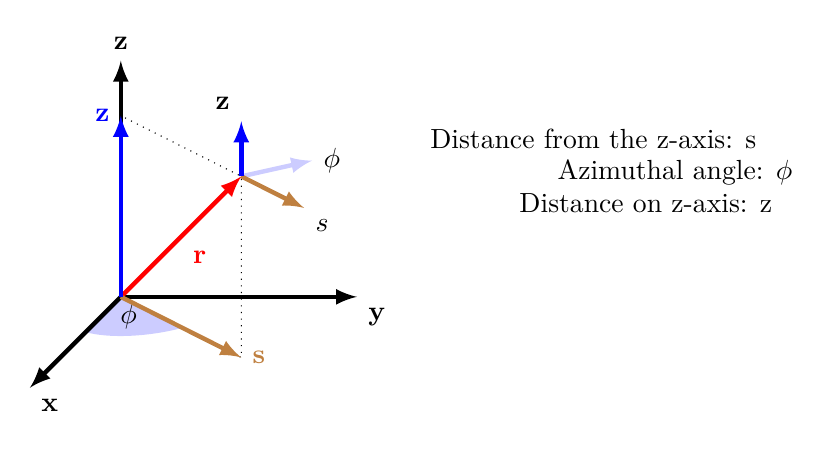
\begin{tikzpicture}  
            \draw [dotted] (0,0,0)--(2.3,0,2)--(2.3,2.3,2)--(0,2.3,0);
            \begin{scope}[canvas is xz plane at y=0]
                \fill [blue!20] (0,0)--(1.2,1) arc [start angle=45, end angle=120,radius=10 mm] node at (0.35,0.65) [black] {$\phi$};
            \end{scope}
            \draw [ultra thick, -latex] (0,0,0)--(3,0,0) node [anchor=north west] {\textbf{y}};
            \draw [ultra thick, -latex] (0,0,0)--(0,3,0) node [anchor=south] {\textbf{z}};
            \draw [ultra thick, -latex] (0,0,0)--(0,0,3) node [anchor=north west] {\textbf{x}};


            \draw [ultra thick, blue!20, -latex] (2.3,2.3,2)--(2.7,2,0.7) node [anchor=west, color=black] {$\e{\phi}$}; 
            \draw [ultra thick, brown, -latex] (2.3,2.3,2)--(3.5,2.3,3.043) node [anchor=north west, color=black] {$\e{s}$}; 
            \draw [ultra thick, blue, -latex] (2.3,2.3,2)--(2.3,3,2) node [anchor=south east, color=black] {$\e{\textbf{z}}$}; 


            \draw [ultra thick, red, -latex] (0,0,0)--(2.3,2.3,2) node at (1,0.5) {\textbf{r}};
            \draw [ultra thick, -latex, brown] (0,0,0)--(2.3,0,2) node [anchor=west] {\textbf{s}};
            \draw [ultra thick, -latex, blue] (0,0,0)--(0,2.3,0) node [anchor=east] {\textbf{z}};


            \node (description text) at (6,2,0) {Distance from the z-axis: s};
            \node at (description text.south) [xshift=29.5, yshift=-5] {Azimuthal angle: $\phi$};
            \node at (description text.south) [xshift=19, yshift=-16] {Distance on z-axis: z};
        \end{tikzpicture}
    \end{figure}
    Important relationships:
    \begin{align*}
        \begin{bmatrix}
        \e{s}\\
        \e{\phi}\\
        \e{z}
        \end{bmatrix}
        &=
        \begin{bmatrix}
        \cos(\phi)&\sin(\phi)&0\\
        -\sin(\phi)&\cos(\phi)&0\\
        0&0&1
        \end{bmatrix}
        \begin{bmatrix}
        \e{x}\\
        \e{y}\\
        \e{z}
        \end{bmatrix}
    \end{align*}
    \begin{center}
    Matrix is orthogonal, transpose to find $\e{x}$ in terms of $\e{s}$
    \vspace{0.5 cm}
    \end{center}
    Position, velocity, and acceleration:
    \begin{align*}
        \vb{r}\qty(s,\phi,z;t)&=
        \begin{bmatrix}
            s(t)
            \\
            \phi(t)
            \\
            z(t)
        \end{bmatrix}
        &
        \vb{v}\qty(s,\phi,z;t)&=
        \begin{bmatrix}
            \dot{s}
            \\
            s\dot{\phi}
            \\
            \dot{z}
        \end{bmatrix}
        &
        \vb{a}\qty(s,\phi,z;t)&=
        \begin{bmatrix}
            \Ddot{s}-r\dot{\phi}^2
            \\
            s\Ddot{\phi}+2\dot{s}\dot{\phi}
            \\
            \Ddot{z}
        \end{bmatrix}
    \end{align*}
    \newpage\noindent
    

\newpage
\subsubsection{Spherical Coordinates}
    In this system of coordinates, the following describe the space's basis set:
    %\tikzsetnextfilename{spherical}
    \tikzfading[name=ball, outer color=transparent!50, inner color=transparent!100]
    \begin{figure}[H]
        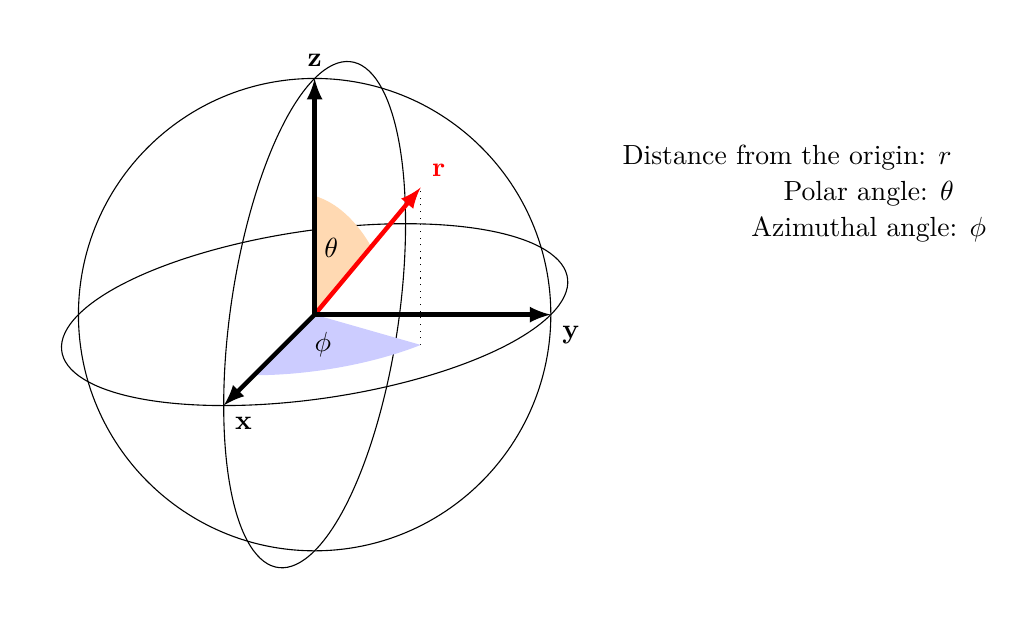
\begin{tikzpicture}
            % 3D is in math convention--> Z sticks out of page in right handed coordinate system. 
            % I relable this to be the physics convention, where Z sticks up. 
            \def\bs{0.3}; % basis scalings
            
            \begin{scope}[canvas is xz plane at y=0]  
                \draw (0,0) circle (3);
            \end{scope}
            \begin{scope}[canvas is xy plane at z=0]  
                \draw (0,0) circle (3);
            \end{scope}
            \begin{scope}[rotate around y=90,canvas is xy plane at z=0]  
                \draw (0,0) circle (3);
            \end{scope}

            %\begin{scope}[canvas is xz plane at y=2]
                % Phi basis vector
                %\draw [ultra thick, blue!20, -latex] (30:2)--++(-45:2*\bs) node [xshift=2, yshift=2,color=black] {\(\e{\phi}\)};
            %\end{scope}
            \begin{scope}[rotate around y=-30,canvas is xy plane at z=0]                
                % Theta arc
                \draw [orange!30, fill=orange!30] (0,0)--(45:15mm) arc [start angle=45, end angle=90,radius=15 mm] node [midway, below, xshift=-5, yshift=-5, black] {\(\theta\)} -- cycle ; 
                
                \draw [ultra thick, red, -latex] (0,0)--(2,2) node [at end, above right] {\(\vb{r}\)};
                \draw [dotted] (2,0)--(2,2); 
                %\draw [ultra thick, orange!30, -latex] (2,2)--(2*\bs+2,-2*\bs+2) node [xshift=1, color=black] {\(\e{\theta}\)};
                %\draw [ultra thick, blue, -latex]      (2,2)--(2*\bs+2,2*\bs+2) node [xshift=1, yshift=3, color=black] {\(\e{r}\)};
            \end{scope}


            \begin{scope}[canvas is xz plane at y=0]
                % Phi angle
                \fill [blue!20] (0,0)--(30:20mm) arc [start angle=30, end angle=90,radius=20 mm]  node [midway, above left] [black] {\(\phi\)} --cycle;
            \end{scope}
        
            \draw [ultra thick, -latex] (0,0,0)--(3,0,0) node [anchor=north west] {\textbf{y}};
            \draw [ultra thick, -latex] (0,0,0)--(0,3,0) node [anchor=south]      {\textbf{z}};
            \draw [ultra thick, -latex] (0,0,0)--(0,0,3) node [anchor=north west] {\textbf{x}};

            \node (r text) at (6,2,0) {Distance from the origin: \(r\)};
            \node (theta text) at (r text.south) [xshift=29.5, yshift=-5] {Polar angle: \(\theta\)};
            \node (phi text) at (theta text.south) [yshift=-5] {Azimuthal angle: \(\phi\)};

        \end{tikzpicture}
    \end{figure}
    Important relationships:
    \begin{align*}
        \begin{bmatrix}
        \e{r}\\
        \e{\theta}\\
        \e{\phi}
        \end{bmatrix}
        &=
        \begin{bmatrix}
        \sin(\theta)\cos(\phi)&\sin(\theta)\sin(\phi)&\cos(\theta)\\
        \cos(\theta)\cos(\phi)&\cos(\theta)\sin(\phi)&-\sin(\theta)\\
        -\sin(\phi)&\cos(\phi)&0
        \end{bmatrix}
        \begin{bmatrix}
        \e{x}\\
        \e{y}\\
        \e{z}
        \end{bmatrix}
    \end{align*}
    \begin{center}
    Matrix is orthogonal, transpose to find $\e{x}$ in terms of $\e{r}$
    \end{center}
    \vspace{0.5 cm}
    Position, velocity, and acceleration:
    \begin{align*}
        \vb{r}\qty(r,\theta,\phi; t)&=
        \begin{bmatrix}
        r(t)
        \\
        \theta(t)
        \\
        \phi(t)
        \end{bmatrix}
        \\
        \vb{v}\qty(r,\theta,\phi;t)&=
        \begin{bmatrix}
        \dot{r}
        \\
        r\dot{\theta}
        \\
        r\sin(\theta)\dot{\phi}
        \end{bmatrix}
        \\
        \vb{a}\qty(r,\theta,\phi;t)&=
        \begin{bmatrix}
        \Ddot{r}-r\dot{\theta}^2-r\dot{\phi}^2\sin^2(\theta)
        \\
        r\Ddot{\theta}+2\dot{r}\dot{\theta}-r\dot{\phi}^2\sin(\theta)\cos(\theta)
        \\
        2r\cos(\theta)\dot{\theta}\dot{\phi}+2\sin(\theta)\dot{r}\dot{\phi}+r\sin(\theta)\Ddot{\phi}
        \end{bmatrix}
    \end{align*}
\newpage      
%\end{document}
	\section{Group Theory}
		\subsection{Lie Groups}
\subsection{SU(2)}
\subsection{SU(3)}
	\section{Lagrangian Mechanics/Classical Field Theory}
		\newpage\subsection{Guiding Principle of Least Action}
Any system of interest can be described in terms of its possible configurations. The different configurations can be parameterized in terms of things like distances, angles, and these parameters describing the system can create a space, which does not need to be the same as physical space. 
\\
The behavior of a pendulum, for example, can be described in terms of the \(x,y,z\) coodrinates of the pendulum in 3D space. As the pendulum moves through time, the coordinates change, always describing where the pendulum is. This can also be explained just as consistently in terms of it's length and angle. If the length of the pendulum doesn't change, then knowing the angle is all that needs to be known. [say something about velocities]
Even it's kinetic and potential energy at any given moment. All of these choices uniquely describe the system, and should be equally valid. 
\\
The quantities used to fully describe the system are the \textbf{generalized coordinates} \(q_i\) (\(i=1,2,3,\ldots)\). Examples of \(q\) could be positions, angles, currents, or even entire fields. Since these coordinates typically evolve in time, the other natural quantities of interest are the generalized velocities \(\dot{q}_i(t)\). 
\begin{center}
	Using the right \(\{q_i(t),\,\dot{q}_i(t)\}\), a system will be fully described at any time \(t\).
\end{center}
The axes of the relevant configuration space are the full set of \(\{q_i(t),\,\dot{q}_i(t)\}\).
The kinetic energy, \(T\), and potential energy, \(U\), of a particle depend on the path taken by the elements of the system in this configuration space.
Average (or even instantaneous) kinetic/potential energies can be regarded as (integral) functionals of their paths. For the simplest example of a single particle that can move in 1-D, taking the generalized coordinates to be the position\footnote{	
	This can be expanded to account for multiple dimensions of generalized coordinates \(\vb{q}=(q_1,\ldots,q_i)\) with a line integral over the parameterized path in configuration space.
	\(\overline{T}=\oo{t_2-t_1} \int_{t_1}^{t_2}T\qty(\vb{q}(t))\,|\dot{\vb{q}}(t)|\dt\)
}:
\begin{align*}
	\overline{T}&=\oo{t_2-t_1} \int_{t_1}^{t_2}\oo{2}m{[\dot{x}(t)]}^2 \dt
	\\
	\overline{U}&= \oo{t_2-t_1} \int_{t_1}^{t_2}U[{x(t)}] \dt
\end{align*}


The definition of the lagrangian can be motivated by describing how the kinetic and potential energies change as the possible paths of the system change. In the explicit case of generalized coordinates being cartesian position and velocity. Describing how \(\overline{T}\) and \(\overline{U}\) change with the functional derivative:

\begin{align*}
	\frac{\delta\overline{T}}{\delta x(t)}
	&=-m\ddot{x}(t)
	\\
	\frac{\delta\overline{U}}{\delta x(t)}
	&=\der{U}{x}
\end{align*}

This change can be more rigorously quantified using the functional derivatives of the two energy functionals: 
\begin{align*}
	m\ddot{x}(t)
	&=-\der{U}{x}
\end{align*}
This is true from physical principles classically.
\begin{align*}
	\frac{\delta\overline{T}}{\delta x(t)}
	&=\frac{\delta\overline{U}}{\delta x(t)}
\end{align*}
\begin{align*}
	\frac{\delta\overline{T}}{\delta x(t)}-\frac{\delta\overline{U}}{\delta x(t)}
	&=0
	\\
	\frac{\delta}{\delta x(t)}\qty(\overline{T}-\overline{U})&=0
\end{align*}
The quantity \(T-V\) is stationary over a classical trajectory, this is what \textit{motivates} the definition of the Lagrangian \(L=T-V\). Using the definitions of \(\overline{T},\,\overline{V}\), it follows that the quantity that is stationary is the time integral of the lagrangian, which is called the action:
\begin{align*}
	\frac{\delta}{\delta x(t)}\qty(\int_{t_1}^{t_2}L\dt)&=0
	\\
	\frac{\delta}{\delta x(t)}\qty(S)&=0
\end{align*}
Out of all possible paths in the configuration space, the path that describes how a physical system evolves in reality will be the path with a stationary action \(S\).


\subsubsection{Moving to Fields}
Fields replace generalized coordinates in field theories.
Instead of \(q_i(t)\) the field is defined at every point in real space \(\phi_i(x,t)\).
Since there is an extra label, \(x\), the lagrangian will also depend on the position derivatives of the field, just like it depended on the time derivatives before. In order to derive the action like before, the 
	\section{Relatevistic Mechanics}
		Lorentz transforms, represented by 4\(\cross\)4 matrices, form a group, where the group operation is matrix multiplication.
\subsection{Lorentz Transforms}
Metric Tensors are used to define distance metrics in 4D spacetime, called spacetime intervals. $g_{\mu\nu}$ is the general metric tensor, and $\eta_{\mu\nu}$ is used for explicitly flat spacetime. For particle physics, either can be used, and it would be understood that $g_{\mu\nu}$ is in flat spacetime. 
\begin{align}
	g_{\mu\nu}&=
	\begin{bmatrix}
		g_{00} & g_{01} & g_{02} & g_{03} \\
		g_{10} & g_{11} & g_{12} & g_{13} \\
		g_{20} & g_{21} & g_{22} & g_{23} \\
		g_{30} & g_{31} & g_{32} & g_{33} \\
	\end{bmatrix}
	\\
	\eta_{\mu\nu}&=\mqty[\dmat[0]{1,-1,-1,-1}]
\end{align}
Four Vectors:
\begin{align*}
	x^{\mu}&=\colvec{ct\\x_{1}\\x_{2}\\x_{3}}=\colvec{ct\\\vb{x}}
	&
	p^{\mu}&=\colvec{cE\\p_{1}\\p_{2}\\p_{3}}=\colvec{cE\\\vb{p}}
	\\[0.5cm]
	A^{\mu}&=\colvec{\oo{c}\phi\\A_{1}\\A_{2}\\A_{3}}=\colvec{\oo{c}\phi\\\vb{A}}
	&
	\pder*[\mu]{}&=\colvec{\oo{c}\pder*{t}\\\pder*{1}\\\pder*{2}\\\pder*{3}}=\colvec{\oo{c}\pder*{t}\\\grad{}}
\end{align*}

Lorentz scalars are invariant under lorentz transformations, this is centrally important, and a Lorentz invariant Lagrangian/Action should be built on Lorentz scalars. This property is encapsulated in a 
frequently used identity, which is obtained by considering the inner product between two four vectors, which is a Lorentz scalar:
\begin{align*}
	a\cdot b&=a^{\mu}\eta_{\mu\nu}b^{\nu}
	\\
	\Big\downarrow\Lambda& \notag \\
	a^{\prime}\cdot b^{\prime}&=a^{\rho}\Lambda^{\mu}_{~\rho}\eta_{\mu\nu} \Lambda^{\nu}_{~\sigma}b^{\sigma}=a\cdot b=a^{\rho}\eta_{\rho\sigma}b^{\sigma}
	\\
	\Lambda^{\mu}_{~\rho}\eta_{\mu\nu} \Lambda^{\nu}_{~\sigma}a^{\rho}b^{\sigma}&=\eta_{\sigma\rho}a^{\rho}b^{\sigma}
\end{align*}
\begin{align}		
	\boxed{\Lambda^{\mu}_{~\rho}\eta_{\mu\nu} \Lambda^{\nu}_{~\sigma}=\eta_{\sigma\rho}}\label{eqn:LorentzMatrixConstraint}
\end{align}
This is a \emph{constraint} on the Lorentz transform matrix.
\\
\(D[\Lambda]^{a}_{~b\,}\) is the matrix representation of the Lorentz Group, and has the properties:
\begin{align*}
	D[\Lambda_1]D[\Lambda_2]&=D[\Lambda_1\Lambda_2]
	\\
	D[\Lambda^{-1}]&=D[\Lambda]^{-1}
	\\
	D[1]&=1
\end{align*}
To find the representations of a group, the typical formulation is to take infinitesimal transformations of the group and to study the resulting algebra. 
\begin{align*}
	\Lambda^{\mu}_{~\nu}=\underbrace{\delta^{\mu}_{~\nu}}_{\rm Identity}+\underbrace{\omega^{\mu}_{~\nu}}_{\rm Infinitesmial}
\end{align*}
From the constraint (\ref{eqn:LorentzMatrixConstraint}), it can be shown that \(\omega^{\mu}_{~\nu}\) must be anti-symmetric, which means there are 6 unique off-diagonal elements, which correspond to the 
\subsubsection{Definitions used in the field (of study):}
Lorentz transforms and causality
\\
spacetime intervals

\subsubsection{Lorentz Transformations of general field}
\begin{align}
	\phi^{a}(\vb{x})&\xrightarrow{\Lambda}\qty(\phi^{a}(\vb{x}))^{\prime}=D[\Lambda]^{a}_{~b\,}\phi^{b}(\Lambda^{-1}\vb{x})
\end{align}
Where \(D[\Lambda]^{a}_{~b\,}\) is the matrix representation of the Lorentz Group.

	\section{Quantum Field Theory}
		\newpage Hamiltonian for harmonic oscillator 
\NewDocumentCommand{\ppp}{}{{\vec{p}\,}}
\begin{equation}
	\hat{\mathcal{H}}=\frac{\hat{p}^2}{2m}+\oo{2}m\omega^2\hat{x}^2\label{eqn:harmonicHamiltonian}
\end{equation}
has the form \(a^2+b^2\) which can be factorized into the product of complex linear terms \((a+ib)(a-ib)\).\\ This would be nice because we could define a single new operator \(\ahat\) that is linear in both \(\hat{x}\) and \(\hat{p}\), and then \(\hat{\mathcal{H}}\) could be written in terms of a single operator (and it's complex conjugate). 
Naively trying this substitution for the harmonic oscillator hamiltonian gives an extra term, since \([\hat{x},\hat{p}]\neq0\). 
\begin{align*}
	\hat{\mathcal{H}}&\neq\hbar\omega\qty(\ahat^{\dagger}\ahat)
	\\
	\hat{\mathcal{H}}&=\hbar\omega\qty(\ahat^{\dagger}\ahat+\frac{1}{2})
\end{align*}
Where
\begin{align*}
	\quad\ahat^{\dagger}&=\sqrt{\frac{m\omega}{2\hbar}}\qty(\hat{x}-\frac{i}{m\omega}\hat{p})\quad \text{(Creation operator)}
	\\
	\quad\ahat      &=\sqrt{\frac{m\omega}{2\hbar}}\qty(\hat{x}+\frac{i}{m\omega}\hat{p})\quad \text{(Annihilation operator)}
\end{align*}
The order can be chosen as \(\ahat^{\dagger}\ahat\) or \(\ahat\ahat^{\dagger}\), but \(\ahat^{\dagger}\ahat\) avoids the IR divergence without needing to subtract the zero point energy, this is why normal ordering chooses the annihilation operators to be on the right.
\\
The generalized coordinate and generalized momentum can be written in terms of the creation/annihilation perator:
\begin{align*}
	\hat{x}&=\sqrt{2\omega}\qty(\ahat+\ahat^{\dagger})
	\\
	\hat{p}&=\sqrt{\frac{\omega}{2}}\qty(\ahat-\ahat^{\dagger})
\end{align*}
Graduating again from generalized coordinates to fields. 
The fields are now written in terms of an infinite linear combination of creation/annihilation operators. Is this because the fields must cover all of space, and the creation/annihilation operators are interpreted as creating states of definite momentum, therefore a fourier expansion can be written (why is that the next step? for localization in space?) \\
\begin{align}
	\phi(\vec{x})&=\int
	\frac{\d^3p}{(2\pi)^3}
	\oo{\sqrt{2E_{\vec{p}}}}
	\qty(
		\ahat_{\ppp}e^{i\vec{p}\cdot\vec{x}}
		+
		\ahat_{\vec{p}}^{\dagger}\,e^{-i\vec{p}\cdot\vec{x}}
	)
	\\
	\pi(\vec{x})&=\int\frac{\d^3p}{(2\pi)^3}
	(-i)\sqrt{\frac{E_{\vec{p}}}{2}}
	\qty(
		\ahat_{\ppp}e^{i\vec{p}\cdot\vec{x}}
		-
		\ahat_{\vec{p}}^{\dagger}\,e^{-i\vec{p}\cdot\vec{x}}
	)
\end{align}
\\
This changes the description subtly. Now in a system with multiple particles, instead of needing to define which particle is in which state, the states are defined in terms of how many particles, or excitations, it has. This is more realistic in QFT because particles themselves are indistinguishable excitations of the same field.
\\
The collection of energy eigenstates makes intuitive sense as an excitation, but since they are momentum/energy eigenstates, they are not localized in space.  

Making this relativistic consistent means properly describing how the field, and therefore the operators, evolve with time. Currently the fields/operators only depend on space, putting them in the Sch\"odinger picture. To change an operator from the Sch\"odinger picture \(\mathcal{O}_{S}\) to Heisenberg \(\mathcal{O}_{H}\) the time evolution is applied to both sides:
\begin{equation}
	\mathcal{O}_{H} = e^{i\hat{\mathcal{H}}t}\mathcal{O}_{S}e^{-i\hat{\mathcal{H}}t}
\end{equation}
This means that the creation/annihilation operators can be made to evolve with time:
\begin{align*}
	\ahat_{\vb{p}}&=e^{i\hat{\mathcal{H}}t}\ahat_{\ppp}e^{-i\hat{\mathcal{H}}t}
	\\
	\ahat_{\vb{p}}&=e^{i\hat{\mathcal{H}}t}\ahat_{\ppp}e^{-i\hat{\mathcal{H}}t}
\end{align*}
This would be a good time to know \(\hat{\mathcal{H}},\ahat^{\dagger}\) commute, check that:
\begin{align}
	\qty[\hat{\mathcal{H}},\ahat^{\dagger}_{\vec{p}}]
	&= \hbar\omega_{\ppp}\ahat^{\dagger}_{\ppp}
	 = E_{\ppp}\ahat_{\vec{p}}^{\dagger}
	\\
	\qty[\hat{\mathcal{H}},\ahat_{\vec{p}}]
	&=-\hbar\omega_{\ppp}\ahat_{\ppp}
	=E_{\ppp}\ahat_{\vec{p}}
\end{align}
Using this commutation relation, a miracle happens and the resulting energies can be substituted in
\begin{align}
	\phi(\vb{x})=\phi(\vec{x},t)&=\int
	\frac{\d^3p}{(2\pi)^3}
	\oo{\sqrt{2E_{\ppp}}}
	\qty(
		\ahat_{\ppp}e^{-i\vb{p}\cdot\vb{x}}
		+
		\ahat_{\vec{p}}^{\dagger}\,e^{i\vb{p}\cdot\vb{x}}
	)\label{eqn:}
	\\
	\pi(\vb{x})=\pi(\vec{x},t)&=\int\frac{\d^3p}{(2\pi)^3}
	(-i)\sqrt{\frac{E_{\vec{p}}}{2}}
	\qty(
		\ahat_{\ppp}e^{-i\vb{p}\cdot\vb{x}}
		-
		\ahat_{\vec{p}}^{\dagger}\,e^{i\vb{p}\cdot\vb{x}}
	)
\end{align}
Since this is now \(\vb{p}\cdot\vb{x}=E_{\ppp}t-\vec{p}\cdot\vec{x}\), the signs flip.
\\
This allows the fields operators \\
For complex scalar fields, Tong defines

\begin{align}
	\psi(\vb{x})&=\int\frac{\d^3p}{\qty(2\pi)^3}
	\oo{\sqrt{2E_{\ppp}}}
	\qty(\bhat_{\ppp}e^{-i\vb{p} \cdot \vb{x}} + \chat_{\ppp}^{\dagger}e^{i\vb{p} \cdot \vb{x}} )
	\\
	\psi^{\dagger}(\vb{x})&=\int\frac{\d^3p}{\qty(2\pi)^3}
	\oo{\sqrt{2E_{\ppp}}}
	\qty(\bhat_{\ppp}^{\dagger}e^{i\vb{p} \cdot \vb{x}} + \chat_{\ppp}e^{-i\vb{p} \cdot \vb{x}} )
\end{align}
Pauli Matrices:
\begin{align*}
	\sigma^1&=\begin{bmatrix} 0 &  1 \\ 1 &  0 \end{bmatrix}&
	\sigma^2&=\begin{bmatrix} 0 & -i \\ i &  0 \end{bmatrix}&
	\sigma^3&=\begin{bmatrix} 1 &  0 \\ 0 & -1 \end{bmatrix}
\end{align*}
Compacted gamma matrices:
\begin{align*}
	\gamma^0&=\begin{bmatrix}0&\mathbb{I}\\\mathbb{I}&0\end{bmatrix}&
	\gamma^i&=\begin{bmatrix}0&\sigma^i\\-\sigma^i&0\end{bmatrix}
\end{align*}
Create a representation of the Lorentz algebra
	\section{Standard Model}
	\section{Particle Physics}
		\subsection{Relatevistic Kinematics of Particles}
\chapter{Experiment (PhD)}
	The divide between theoretical math and experimental application became hard to quantify (Looking at \(p_T,\eta\) spectra is invaluble for an analysis, but when learning about Lorentz transforms, \(\eta\) is just a rotation, and no one cares about \(p_T\)), so I divided them by the amount of specialization. The first chapter is building to particle physics as a whole, this is focusing just on particle physics, specifically how it exists as a practice. Including more focus on electroweak (EW) physics and two Higgs doublet model (2HDM).
	\section{ATLAS Detector}
	\section{Components of a General Particle Detector}
	\section{History of Particle Physics}
	\section{ATLAS Analysis}
		\subsection{Particle Physics}
\newpage
\includepdf[height=0.5\pdfpageheight, pagecommand={\thispagestyle{fancy}}]{Experiment/Particle/build/ParticleTimeline.pdf}
\newpage
\begin{itemize}
	\item Transverse momentum \pT:\@\ momentum transverse to the beam axis.
	\item Transverse Energy \ET:\@\ Energy transverse to beam axis, deposited in calorimeter.
	\item Scalar Fields
	\item Classical Scattering
	\item ATLAS Data
	\begin{itemize}
		\item Run 1: 2010--2012
		\item Run 2: 2015--2018
		\item Run 3: 2022--2026
	\end{itemize}
	\item Cutflow: Volume of phase space (number of events) after each cut is applied. Used to visualize the cut restrictions as they are applied. 
	\item Validation Region / Control Region: A selection of data space that very close to signal selection region. Used to `validate' the background region. Usually just has same cuts as signal region with exception of one cut inverted.
	\item Quantization
	\item On-shell: 
	\item Branching Ratio: The fraction of particles that decay via a particular decay mode.
	\item Cross Section: A measure of the probability that a specific process will occur when particles
	      collide. It is typically measured in units of area, such as barns (1 barn = $\rm 10^{-28} m^2$ = $\rm 10^{-24} cm^2$).
	\item Luminosity: A measure of the number of particles per unit area per unit time in a collider. It is used to calculate the event rate for a given process.  \(L=\oo{\sigma}\der{N}{t}\)
	\item Integrated Luminosity: The total luminosity accumulated over a specific period of time. It is often expressed in inverse femtobarns (\(\rm fb^{-1}\)).
	\item Event Topologies:
\end{itemize}
\subsection{Width}
When particles decay immeasurably fast (\W, \Z, \h, t), width $\Gamma$ is used instead of mean lifetime $\tau$. 
\subsection{Higgs}
The Higgs boson \h\ explains how the vector bosons get their mass (why it's \W, \Z and $\gamma$) instead of all or none having mass. 
The \h\ also explains how fermions get their mass, and there is a correspoondance between Newtons first law. Interacting with the higgs field makes it difficult for a body to accelerate, which is analogous to inertia.
\subsection{Gamma Matrix Identities}
	\begin{minipage}{0.45\textwidth}
		\begin{align*}
			\gamma^{0\dagger}&=\gamma^0
			\\
			\gamma^{j\dagger}&=-\gamma^j\quad\qty(j=1,2,3)
			\\
			\gamma^0\gamma^{\mu\dagger}\gamma^0&=\gamma^\mu
			\\
			\gamma^{0}\gamma^{0}&=\mathbb{I}
			\\
			\gamma^\mu\gamma_\mu&=4
			\\
			\gamma^\mu\gamma_\nu\gamma_\mu&=-2\gamma_\nu
			\\
			\gamma^\mu a_\mu&=\gamma_\mu a^\mu=\slsh{a}
			\\
			\psi^\dagger\gamma^0&=\bar{\psi}
		\end{align*}
	\end{minipage}
	\begin{minipage}{0.48\textwidth}
		\begin{align*}
			\qty{\gamma_\mu,\gamma_\nu}&=\gamma_\mu\gamma_\nu+\gamma_\nu\gamma_\mu=2g_{\mu\nu}
			\\
			\gamma^\mu\gamma_\mu&=4
			\\
			\qty[\gamma^\mu,a_\mu]&=0
			\\
			\gamma^\mu a_\mu&=\gamma_\mu a^\mu=\slsh{a}
			\\
			\Tr(\mathbb{I})&=4
			\\
			\Tr(\gamma_\mu\gamma_\nu)&=\Tr(\gamma^\mu\gamma^\nu)=4
			\\
			\Tr(\gamma^\mu\gamma^\nu\gamma^\rho\gamma^\sigma)&=4(g^{\mu\nu}g^{\rho\sigma}-g^{\mu\rho}g^{\nu\sigma}+g^{\mu\sigma}g^{\nu\rho})
		\end{align*}
	\end{minipage}
	\\[0.25 cm]
	Gamma 5 matrix:
	\\
	\begin{minipage}{0.45\textwidth}
		\begin{align*}
			\gamma_5^\dagger&=\gamma_5
			\\
			\gamma_{5}\gamma_{5}&=\mathbb{I}
			\\
			\qty{\gamma_5,\gamma_\nu}&=0
			\\
			\Tr(\gamma_5)&=0
			\\
			\Tr(\gamma_\mu\gamma_5)&=0
			\\
			\Tr(\gamma_\mu\gamma_\nu\gamma_5)&=0
			\\
			\Tr(\gamma_\mu\gamma_\nu\gamma_\rho\gamma_5)&=0
			\\
			\Tr(\gamma_\mu\gamma_\nu\gamma_\rho\gamma_\sigma\gamma_5)&=4i\epsilon_{\mu\nu\rho\sigma}
		\end{align*}
	\end{minipage}
	\begin{minipage}{0.45\textwidth}
		\begin{align*}
			P_L&=\frac{1-\gamma_5}{2}
			\\
			P_R&=\frac{1+\gamma_5}{2}
			\\
			P_L\gamma_\mu&=\gamma_\mu P_R
			\\
			P_L(\gamma^\mu\gamma^\nu\dotsc\text{odd})P_L&=0
			\\
			P_L(\gamma^\mu\gamma^\nu\dotsc\text{even})P_L&=P_L\qty(\gamma^\mu\gamma^\nu\dotsc)
		\end{align*}
	\end{minipage}
	\\[0.25 cm]
\subsection{Spinor Identities:}
	\begin{equation*}
		u^s(\vb{p})=
		\begin{pmatrix}
			\ \sqrt{p\cdot\sigma}\xi^{s}\ 
			\\
			\ \sqrt{p\cdot\overline{\sigma}}\xi^{s}\ 
		\end{pmatrix}
		\qquad\qquad
		v^s(\vb{p})=
		\begin{pmatrix}
			\ \sqrt{p\cdot\sigma}\xi^{s}\ 
			\\
			\ -\sqrt{p\cdot\overline{\sigma}}\xi^{s}\ 
		\end{pmatrix}
	\end{equation*}
	Inner Products:
	\begin{align*}
		u^r(\vb{p})^\dagger\cdot u^s(\vb{p})&=2p_0\delta^{rs}
		&
		v^r(\vb{p})^\dagger\cdot v^s(\vb{p})&=2p_0\delta^{rs}
		\\
		\overline{u}^r(\vb{p})\cdot u^s(\vb{p})&=2m\delta^{rs}
		&
		\overline{v}^r(\vb{p})\cdot v^s(\vb{p})&=-2m\delta^{rs}
	\end{align*}
	Outer Products:
	\begin{align*}
		\sum_{s=1}^{2}u^s(\vb{p})\bar{u}^s(\vb{p})&=\slsh{p}+m
		&
		\sum_{s=1}^{2}v^s(\vb{p})\bar{v}^s(\vb{p})&=\slsh{p}-m
	\end{align*}
	\begin{align*}
		\qty(\overline{u}\gamma^\mu v)^*&=\bar{v}\gamma^\mu u 
		\\
		\qty(\overline{u}\gamma^\mu P_Lv)^*&=\bar{v}\gamma^\mu P_L u
	\end{align*}
\newpage
\subsection{Mandelstam Variables}

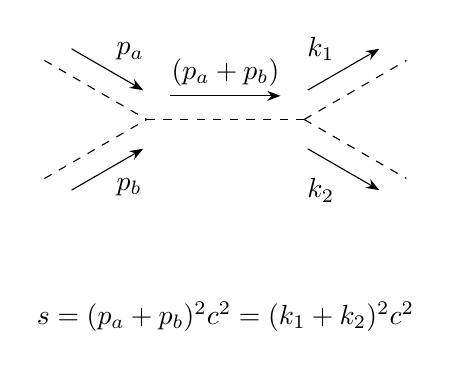
\begin{tikzpicture}[baseline=(current bounding box.south)]% S CHANNEL Template diagram. 
    % Template diagrams are labelled from top to bottom, going left to right. 
    % p_{a,b,c,...} are incoming,
    % k_{1,2,3,...} are outgoing,
    % v_{1,2,3,...} are vertices. 
    \def\propAngle{0}% angle of virtual propagators (from horizontal)
    \def\pAngle{30}% angle of incoming particle (from horizontal)
    \def\kAngle{30}% angle of outgoing particle (from horizontal)
    \def\legLength{1.5}% length of external leg
    \def\propLength{2}% length of propagator

    \begin{feynman}
        \vertex (v_1) at (0,0);
        \vertex (v_2) at ($(v_1)+(\propAngle:\propLength)$);

        \vertex (p_a) at ($(v_1)-(-\pAngle:\legLength)$);
        \vertex (p_b) at ($(v_1)-( \pAngle:\legLength)$);
        \vertex (k_1) at ($(v_2)+( \kAngle:\legLength)$);
        \vertex (k_2) at ($(v_2)+(-\kAngle:\legLength)$);

        \draw[scalar, momentum=\((p_a+p_b)\)] (v_1) -- (v_2);
        
        \draw[scalar, momentum=\(p_a\)]  (p_a) -- (v_1);
        \draw[scalar, momentum'=\(p_b\)] (p_b) -- (v_1);
        \draw[scalar, momentum=\(k_1\)]  (v_2) -- (k_1);
        \draw[scalar, momentum'=\(k_2\)] (v_2) -- (k_2);
    \end{feynman}
	\node at ($(v_1)! 0.5!(v_2)-(0,\legLength+1)$) {\(s=(p_a+p_b)^2c^2=(k_1+k_2)^2c^2\)};% below, midway between v_1 and v_2
\end{tikzpicture}
~~
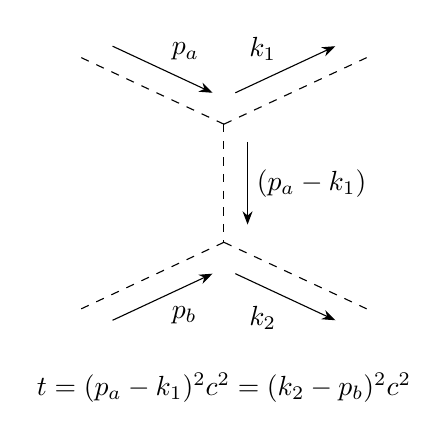
\begin{tikzpicture}[baseline=(current bounding box.south)]% T CHANNEL Template diagram. 
    % Template diagrams are labelled from top to bottom, going left to right. 
    % p_{a,b,c,...} are incoming,
    % k_{1,2,3,...} are outgoing,
    % v_{1,2,3,...} are vertices. 
    \def\propAngle{0}% angle of virtual propagators (from vertical)
    \def\pAngle{25}% angle of incoming particle (from horizontal)
    \def\kAngle{25}% angle of outgoing particle (from horizontal)
    \def\legLength{2}% length of external leg
    \def\propLength{1.5}% length of propagator
    
    \begin{feynman}
        \vertex (v_1) at (0,0);
        \vertex (v_2) at ($(v_1)+(\propAngle-90:\propLength)$);

        \vertex (p_a) at ($(v_1)-(-\pAngle:\legLength)$);
        \vertex (k_1) at ($(v_1)+( \kAngle:\legLength)$);
        \vertex (p_b) at ($(v_2)-( \pAngle:\legLength)$);
        \vertex (k_2) at ($(v_2)+(-\kAngle:\legLength)$);

        \draw[scalar, momentum=\(p_a\)] (p_a) -- (v_1);
        \draw[scalar, momentum=\(k_1\)] (v_1) -- (k_1);

        \draw[scalar, momentum=\((p_a-k_1)\)] (v_1) -- (v_2);
        
        \draw[scalar, momentum'=\(p_b\)] (p_b) -- (v_2);
        \draw[scalar, momentum'=\(k_2\)] (v_2) -- (k_2);
    \end{feynman}
	\node at ($(p_b)! 0.5!(k_2)-(0,1)$) {\(t=(p_a-k_1)^2c^2=(k_2-p_b)^2c^2\)};% below, midway between p_b and k_2
\end{tikzpicture}
~~
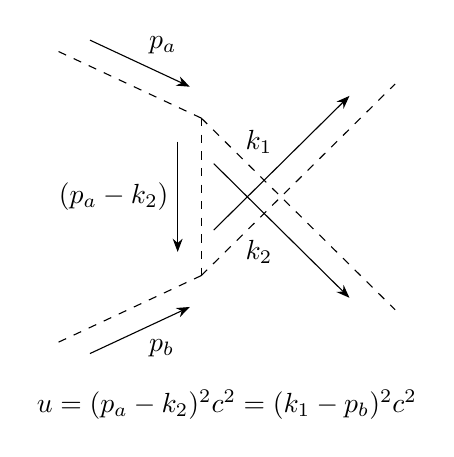
\begin{tikzpicture}[baseline=(current bounding box.south)]% U CHANNEL Template diagram. 
    % Template diagrams are labelled from top to bottom, going left to right.
    % p_{a,b,c,...} are incoming,
    % k_{1,2,3,...} are outgoing,
    % v_{1,2,3,...} are vertices. 
    \def\propAngle{0}% angle of virtual propagators (from vertical)
    \def\pAngle{25}% angle of incoming particle (from horizontal)
    \def\kAngle{10}% angle of outgoing particle (from horizontal)
    \def\legLength{2}% length of external leg
    \def\propLength{2}% length of propagator
    
    \begin{feynman}
        \vertex (v_1) at (0,0);
        \vertex (v_2) at ($(v_1)+(\propAngle-90:\propLength)$);

        \vertex (p_a) at ($(v_1)-(-\pAngle:\legLength)$);
        \vertex (k_1) at ($(v_1)+( \kAngle:\legLength+0.5)$);
        \vertex (p_b) at ($(v_2)-( \pAngle:\legLength)$);
        \vertex (k_2) at ($(v_2)+(-\kAngle:\legLength+0.5)$);

        \draw[scalar, momentum=\(p_a\)] (p_a) -- (v_1);
        \draw[scalar, momentum'=\(k_2\)] (v_1) -- (k_2);

        \draw[scalar, momentum'=\((p_a-k_2)\)] (v_1) -- (v_2);
        
        \draw[scalar, momentum'=\(p_b\)] (p_b) -- (v_2);
        \draw[scalar, momentum=\(k_1\)] (v_2) -- (k_1);
    \end{feynman}
	\node at ($(p_b)! 0.5!(k_2)-(0,1)$) {\(u=(p_a-k_2)^2c^2=(k_1-p_b)^2c^2\)};% below, midway between p_b and k_2
\end{tikzpicture}

\newpage
%\subsection{Feynman Rules}
%	\tikzfeynmanset{
%		every vertex={red},
%		every particle={blue},
%		every blob={draw=black, pattern color=black},
%		}
%	\begin{align*}
%		%Incoming anti/fermions
%		\feynmandiagram[small, baseline=(v1.base), horizontal=v1 to v2]
%		{
%			v1 [color=black, particle=$f$] -- [fermion] v2[blob]-- [draw=none] v3 [particle={\phantom{$f$}}, color=white]
%		};
%		&\quad\longleftrightarrow\quad
%		u(p,s)
%		\\
%		\feynmandiagram[small, baseline=(v1.base), horizontal=v1 to v2]
%		{
%			v1 [color=black, particle=$f$] -- [anti fermion] v2[blob]-- [draw=none] v3 [particle={\phantom{$f$}}, color=white]
%		};
%		&\quad\longleftrightarrow\quad
%		\overline{v}(p,s)
%		\\
%		% Outgoing anti/fermions
%		\feynmandiagram[small, baseline=(v1.base), horizontal=v1 to v2]
%		{
%			v3 [draw=none] -- [draw=none] v1 [blob] -- [fermion] v2 [color=black, particle=$f$]
%		};
%		&\quad\longleftrightarrow\quad
%		\overline{u}(p,s)
%		\\
%		\feynmandiagram[small, baseline=(v1.base), horizontal=v1 to v2]
%		{
%			v3 [draw=none] -- [draw=none] v1 [blob] -- [anti fermion] v2 [color=black, particle=$f$]
%		};
%		&\quad\longleftrightarrow\quad
%		v(p,s)
%		\\
%		% Photon fermion interaction
%		\feynmandiagram[small, baseline=(v1.base), horizontal=v1 to v2]{
%		v1 [particle=$\mu$, color=black] -- [photon] v2,
%		[particle=$f$] a -- [fermion] v2 -- [fermion] b [particle=$f$],
%		};
%		&\quad\longleftrightarrow\quad
%		-iQ_fe\gamma^{\mu}
%	\end{align*}%
	% include all references in bibliography regardless of if they've been cited
%\nocite{*}
%\printbibliography
\end{document}